%\documentclassreport]{jsbook}
\documentclass[report, 11pt]{jsbook}
\usepackage[dvipdfmx]{graphicx}
\usepackage{okumacro}
\usepackage{ascmac}
\usepackage{url}
%\usepackage{listings,jlisting}
\usepackage{listings}%,jlisting}
\usepackage{slashbox}

\lstset{
    language=Java,
    basicstyle=\ttfamily\scriptsize,
    commentstyle=\textit,
    classoffset=1,
    keywordstyle=\bfseries,
    frameround=tttt,
    frame=single,
    framesep=5pt,
    showstringspaces=false,
    numbers=left,
    breaklines=true,
    stepnumber=1,
    numberstyle=\scriptsize,
    tabsize=2,
    xrightmargin=0zw,
    xleftmargin=0zw,
}


\setcounter{tocdepth}{2}

%\setcounter{secnumdepth}{5}
%\makeatletter
%\newcommand{\subsubsubsection}{\@startsection{paragraph}{4}{\z@}%
%    {1.5\baselineskip \@plus.5\dp0 \@minus.2\dp0}%
%    {.5\baselineskip \@plus2.3\dp0}%
%    {\reset@font\normalsize\bfseries}
%}
%\newcommand{\subsubsubsubsection}{\@startsection{subparagraph}{5}{\z@}%
%    {1.5\baselineskip \@plus.5\dp0 \@minus.2\dp0}%
%    {.5\baselineskip \@plus2.3\dp0}%
%    {\reset@font\normalsize\itshape}
%}
%\makeatother
%\setcounter{tocdepth}{5}

\begin{document}

\pagestyle{empty}

\begin{center}

\vspace{5cm}

\textbf{\Large 卒業論文2014年度(平成26年度)}

\vspace{1cm}

\textbf{\LARGE 無線センサネットワークにおけるオペレーティングシステムに対する動的なスケジューリングスイッチング機構}
%\vspace{2cm}
\vspace{3cm}

\textbf{\underline{\large 指導教員}}\\
\textbf{慶應義塾大学環境情報学部}

\textbf{\Large 徳田 英幸}\\
\textbf{\Large 村井 純}\\
\textbf{\Large 楠本 博之}\\
\textbf{\Large 中村 修}\\
\textbf{\Large 高汐 一紀}\\
\textbf{\Large Rodney D. Van Meter III}\\
\textbf{\Large 植原 啓介}\\
\textbf{\Large 三次 仁}\\
\textbf{\Large 中澤 仁}\\
\textbf{\Large 武田 圭史}

\vspace{6cm}

\textbf{\LARGE 慶應義塾大学 環境情報学部}

\vspace{.5em}

\textbf{\LARGE 小町 芳樹}

\vspace{.3em}

\textbf{\it ysk@ht.sfc.keio.ac.jp}



\newpage

\end{center}

\pagestyle{plain}


\frontmatter
\begin{center}
\textbf{\Large 卒業論文要旨 2014年度(平成26年度)}

\vspace{6.18mm}

\textbf{\Large 無線センサネットワークにおけるオペレーティングシステムに対する動的なスケジューリングスイッチング機構}
\end{center}

\vspace{10mm}
近年技術の発展によりセンサノードの低価格化,高性能化が進み,
それに伴い,ネットワークに繋がる物理センサが自動的に多様なデータをやり取りし,
それらを様々な形で活用する無線センサネットワークが普及しつつある.
主にその結果は,環境モニタリングやターゲットトラッキングにおいて
顕著に表れており,センサネットワークが我々を支える生活基盤となり得る将来は遠くはない.

無線センサネットワークにおけるオペレーティングシステムは
イベントモデルとスレッドモデルに分類できるが,
%環境モニタリングやターゲットトラッキングなどの
リアルタイム性のある処理が
長期間にわたって行われるような環境では,
それらのモデルのどちらかを選択することは望ましくない.
Dunkelsらの開発したContiki\cite{Dunkels:2004:CLF:1032658.1034117}
では,
Protothreads\cite{Dunkels:2006:PSE:1182807.1182811}
というシステムを採用することで,
%イベントモデルでありながらもスレッドモデルのようなプログラムの記述を実現している.
イベントモデルでありながらもスレッドモデルと同様の挙動を行うことができる.
しかしながら,Protothreadsを採用した場合でも,
タスク実行中にさらに優先度の高いタスクの実行を要請された際に,
スレッドモデルのように割り込みをし,タスクを切り替えることはできないのが現状である.

本研究では,Protothreadsを利用し,
上記ような時間的制約を伴ったイベントが発生する環境における,
省電力なオペレーティングシステムについて提案する.
本システムは通常イベントモデルとしてタスクの実行を行うことで省電力を実現し,
リアルタイム性の必要なタスク発生時には割り込みを発生させ,
優先的にそのタスクの処理を行うことを可能にしている.
最後に本システムの性能を評価し,有用性を証明する.


\vspace{10mm}
キーワード :\\
\hspace{3.5em}無線センサネットワーク,環境モニタリング,ターゲットトラッキング,オペレーティングシステム,リアルタイム処理

\begin{flushright}
\textbf{慶応義塾大学環境情報学部}\\
\textbf{小町 芳樹}
\end{flushright}

\newpage

\begin{center}
\textbf{\Large Abstract of Bachelor's Thesis}
\textbf{\Large Academic Year 2014}
\vspace{6.18mm}

\textbf{\Large A Dynamic Scherduling System for Operating Systems in Wireless Sensor Networks}
\end{center}

\vspace{10mm}

In recent years, 
developed technology made 
sensor nodes cheaper and high performance.
As a result of this advanced technology, 
Wireless Sensor Networks (WSN) 
in which physical sensors connected with networks
automatically transmit and receive various data 
are constantly growing and used in various ways.
In particular, the results are most remarkable
in environmental monitoring and target tracking.
In the future, WSN will become the foundation of our life supporting. 

Operating Systems (OS) in WSN
are divided into events model and threads model.
However, it is undesireble to 
select OS from these models  
in environments where 
real time tasks have been processed 
for a long period.
%for a long period,
%such as environmental monitoring and target tracking.
We can program applications easily
with OS
in events model which
has the characteristics of threads model
by using Protothreads\cite{Dunkels:2006:PSE:1182807.1182811} 
in Contiki\cite{Dunkels:2004:CLF:1032658.1034117}
proposed by Dunkels et al.
However, 
if a task which has more priority was posted 
while another task has been processed,
the processed task cannot be interrupted,
%and we cannot switch the processed task to the arrived task 
and the processed task cannot be switched to the arrived task 
with Protothreads
in the existing circumstances.

In this research, we propose an energy-efficient operating system 
using Protothreads
in environments where events with time constraint occurred.
In this system,
tasks are usually executed as general events model OS, 
which saves energy.
If an event which requires real time processing occurred,
current task will be interrupted and 
real time task will be dealt with as priority.
Finally, we evaluate this system and prove feasibility.


\vspace{10mm}
Keywords :\\
\hspace{3.5em}Wireless Sensor Networks, Environmental Monitoring, Target Tracking, Operating Systems, Real Time Processing 
\begin{flushright}
\textbf{Yoshiki Komachi}\\
\vspace{5mm}
\textbf{Faculty of Environment and Information Studies}\\
\textbf{Keio University}
\end{flushright}

\tableofcontents
\listoffigures
\listoftables

\mainmatter
\chapter{序論}
\begin{large}
\begin{quote}
%本章では,まずセンサデータの増加などの本研究の背景を述べ,次いで,センサデータの公衆一般化において発生する問題の解決という本研究の目的について言及し,最後に本論文の構成を示す.
本章では,まず
無線センサネットワークオペレーティングに関する本研究の背景を述べ,
次いで,
%センサデータの公衆一般化において発生する問題の解決という
オペレーティングシステムのモデル選択において
発生する問題の解決という
本研究の目的について言及し,
最後に本論文の構成を示す.
\end{quote}
\end{large}
\clearpage

\section{本研究の背景}
近年センサの低価格化,高性能化により,センサネットワークが普及し,
それに伴いセンサ用のオペレーティングシステムの研究も発展を遂げている.
センサネットワークのオペレーティングシステムには主に2種類あり,
省資源性かつ低オーバヘッドを実現したイベントモデルと,
リアルタイム処理を可能としたマルチスレッドモデルが存在している.
センサネットワーク用のオペレーティングシステムではイベントモデルが主流となっている.

イベント駆動型のTinyOSは,省資源かつ低オーバヘッドの実現に成功しているが,
リアルタイム処理を行うことができていない.
また,言語もnesCという特殊な言語を使用しているため,
プログラムが非常に書きにくいという欠点も存在する.
それに対して,Nano-RKはリアルタイム処理をサポートしているが,
イベント駆動型のオペレーティングシステムと比較すると資源の消費が大きく,
高オーバヘッドである.

Contikiはイベント駆動型のオペレーティングシステムで,使用言語はC言語である.
ContikiはProtothreadsと呼ばれるメカニズムを使用しており,
イベント駆動型でありながらスレッドの切り替えを行うことができる.
そのため,イベント駆動型の特徴となっているプログラムの書きにくさを解消することに成功している.
しかし,タスクを処理する優先順位を明確に決める手法が定められていないため,
タスクの切り替えはできるが,未だにリアルタイム処理は不可能なのが現状である.


\section{本研究の目的}
Contikiはイベント駆動型でありながら,
マルチスレッドでタスクを変更することができるため,
リアルタイム処理と親和性があると推測できる.
本研究では,Contikiにスケジューラを実装し,
省資源性かつ低オーバヘッドでありながら,
リアルタイム処理の可能なオペレーティングシステムの実現を目的とする.
%最後に,本システムの評価を行うとともに,有用性を証明する.


%多次元データに対して,センサデータの時間的特殊性を考慮した,T-Ringという分散管理手法を提案し,管理について,利用するアプリケーションの特徴を幾つかの軸で分類し,既存の手法を用いたシステムがどのようなアプリケーションに適するのかを明らかにする.次に,センサデータの時間的特殊性を考慮したシステムが必要なアプリケーションを提示する.最後に,センサデータの時間的特殊性を考慮したシステムの提案し,パフォーマンスの低下を防ぐ.

\section{本論文の構成}
%本論文では,2章において,センサネットワークの一般公衆化とアプリケーションの分類から,そのデータ管理において必要な機能要件を示し,センサデータの時間的特殊性について述べる.3章では,センサデータではない公衆コンテンツの管理とDHTを用いた広域公衆センサデータについての関連研究を紹介する.4章,5章では,センサデータの時間的特殊性に着目したデータ管理システムを示す.6章で,提案手法に対する評価を行い,7章で本研究のまとめを行う.

本論文では,
2章において,無線センサネットワークにおけるアプリケーションを分類し,
それぞれにおける特徴について議論する.
3章では,無線センサネットワークにおけるオペレーティングシステムについて紹介し,
各システムについて比較を行う.
4章で,無線センサネットワークにおけるモデル選択に関する問題点について言及し,
5章では,その問題を解決する手法について,設計と実装の観点から考察する.
6章にて,提案手法に対する評価を行い,7章で本研究のまとめを行う.


\chapter{無線センサネットワーク}
\begin{large}
\begin{quote}
本章では,最初に無線センサネットワークについて導入する.
次に本研究の想定環境である,
環境モニタリングとターゲットトラッキングについてそれぞれ例を提示し,
%無線センサネットワークにおける,
エネルギーの節約とリアルタイム処理の必要性について述べる.
\end{quote}
\end{large}
\clearpage

\section{はじめに}
近年,小型センサの発展を促すセンサ微小電気機械システム技術の進歩により,
無線センサネットワークが急速に普及してきている.
無線センサネットワークで使用されるノードは非常に小さく,
処理機能や計算リソースが制限されているものの,
%数年前と比べて安価な値段で購入できるようになった.
%これらのセンサノードはセンシング,
センシング,計測,情報収集能力,
そしてユーザに対してセンシングしたデータを転送する機能でさえも
備えている.
%近年技術の発展によりセンサノードの低価格化,高性能化が進み,
%それに伴い,ネットワークに繋がる物理センサが自動的に多様なデータをやり取りし,
%それらを様々な形で活用する無線センサネットワークが普及してきている.
代表的なセンサノードとして,Iris Mote\cite{irismote}
やMicaZ\cite{Hill:2002:MWP:623308.624560},
SunSPOT\cite{sunspot}などがある.

Iris Moteは図\ref{fig:iris_mote}のようなものであり,
アメリカのCrossbow Technology社が開発したセンサネットワーク用の無線端末である.
それに対して,MicaZはカリフォルニア大学バークレー校における
スマートダストプロジェクト\cite{Kahn:1999:NCC:313451.313558}によって開発された.
ハードウェア,オペレーティングシステム,開発言語,シミュレータ,
ライブラリといったアプリケーション開発環境を提供しており,
アプリケーション開発が容易であるため,
現在センサネットワークの研究で多く使用されている.
図\ref{fig:micaz}にMicaZの写真を示す.
MicaZは小型なため,様々な場所に応用することができる.
%SunSPOTは図\ref{fig:sunspot}のようなものであり,
%サン・マイクロシステムズが開発した
%IEEE 802.15.4に準拠した無線センサーネットワークデバイスである.
%SunSPOTとはSun Small Programmable Object Technologyの略称であり,
%Javaで実装することができるため,初心者でも扱いやすいセンサデバイスとなっている.
SunSPOTはSun Small Programmable Object Technologyの略称で知られる,
図\ref{fig:sunspot}のような
無線センサネットワークデバイスであり,
Javaで実装することができるため,初心者でも扱いやすいセンサデバイスとなっている.


\begin{figure}[htbp]
 \begin{minipage}{0.5\hsize} \begin{center}
     
\includegraphics[width=40mm]{./images/iris_mote.eps}
    \end{center}
    \caption{Iris Mote}
    \label{fig:iris_mote}
 \end{minipage}
 \begin{minipage}{0.5\hsize}
    \begin{center}
     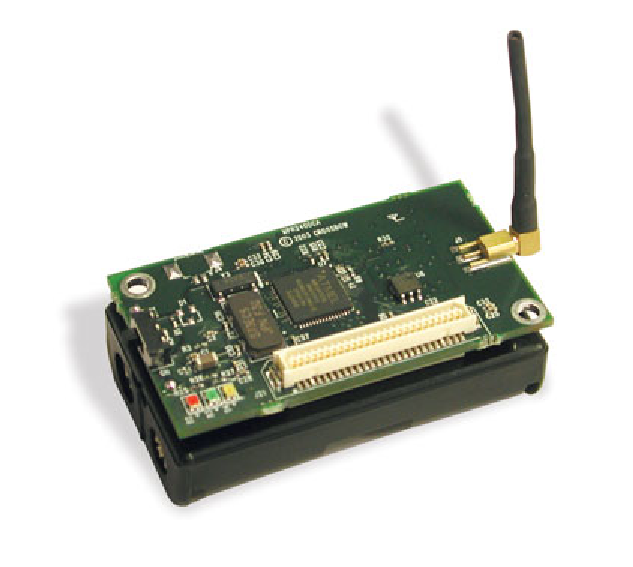
\includegraphics[width=45mm]{./images/micaz.eps}
    \end{center}
    \caption{MicaZ}
    \label{fig:micaz}
 \end{minipage}
\end{figure}

\begin{figure}[htbp]
 \begin{center}
  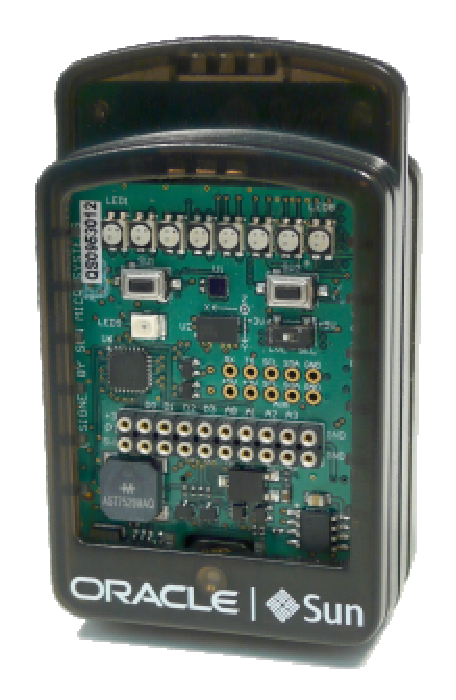
\includegraphics[width=20mm]{./images/sunspot.eps}
 \end{center}
 \caption{SunSPOT}
 \label{fig:sunspot}
\end{figure}


無線センサネットワークアプリケーションを分類した場合,
図\ref{fig:overview_of_sensor_applications}のように
環境モニタリングとターゲットトラッキングの大別される
\cite{Yick:2008:WSN:1389582.1389832}.
環境モニタリングとターゲットトラッキングについてはそれぞれ,
\ref{sec:environmental_monitoring}と
\ref{sec:target_tracking}にて詳細に解説する.


\begin{figure}[htbp]
 \begin{center}
  \includegraphics[width=150mm]{./images/overview_of_sensor_applications.eps}
 \end{center}
 \caption{センサアプリケーションの概要}
 \label{fig:overview_of_sensor_applications}
\end{figure}




\section{環境モニタリング}\label{sec:environmental_monitoring}
環境モニタリングの歴史は長く,
かつては手動によりデータの収集を行っていたが,
デジタルデータロガーの普及により,
より安く,容易にデータの授受を行うことができるようになった.
しかしながら,環境モニタリングでは大抵の場合,
対象となる範囲全域での監視が求められていることに対して,
デジタルデータロガーを利用した場合,
ある一点においてのみのモニタリングしか行うことができなかったため,
デジタルデータロガーに代わる
環境モニタリングの次なる手段として,
無線センサネットワークが採用され始めている.
センサノードには様々なセンサが搭載されており,
センサノードを対象とする地域に配置し,
ネットワークを構築することで,
デジタルデータロガーでは成し得なかった,
広範囲におけるモニタリングを可能としている.

無線センサネットワークを用いた環境モニタリングでは,
モニタリング対象の行動に変化があった際には,
それに応じたタスクを優先的に行わなければならない.
このような時間的制約を伴ったタスクの処理が必要なアプリケーションを想定した場合,
オペレーティングシステムとして
リアルタイム処理を行うことが可能なものを選択することが多い.
無線センサネットワークにおけるオペレーティングシステムのリアルタイム性については,
\ref{sec:threads_model}において詳細に述べる.
本節では代表的な環境モニタリングとして,
森林火災検知と野生動物の生態調査を例に挙げる.




\subsection{森林火災検知}
%\vspace{0.5em}
森林火災は原生林において生じる制御不可能な火災であり,
自然資源と人的資源の両者に多大な被害を与える.
具体的に,木々を根絶やし,基盤となる施設を燃やし,
さらには都市部付近における死亡者数を増加させてしまう場合も少なくない.
森林火災の共通の原因として,落雷や人間の不注意,
そして燃料の野ざらしによる極度の乾燥などが挙げられる.
火災は森林の生態系の一部としてみなされることもあるが,
ほとんどの場合において,
火災により発生する公衆安全や自然資源に対するダメージは耐え難いものであり,
被害を最小限に抑えるためにも火災の早期発見と鎮圧が極めて重要である.
%森林火災検知システムにおいて,
%災害の規模を最小化するために即座に対応することが最も重要であることは既に述べたが,
しかしながら低解像度かつ長期走査により,
%現在の
中規模もしくは大規模火災監視システムは適時検知を行うことは困難であり,
高精度のリアルタイム火災検知を提供できる拡張性のある手法が求められていた.

近年無線センサネットワークにおける発展が著しく,
森林火災を検知する際に役立つ,温度,相対湿度,さらに煙などの
様々な現象をセンシングすることが可能であることから,
無線センサネットワークがこれらの問題を解決できる手法として関心を集めている.
%リアルタイム森林検知システム構築するための将来有望なフレームワークを構築.
%近い将来,
%森林火災検知のための
%様々なセンシングモジュールが明確にデザインされ,
%最適化される.
%加えて,
火災が発生している間,定期的な監視を実現するために,
センサノードは数週間にわたってオペレーションをすることが可能であり,
%航空機を利用することで,
森林火災によって生じる被害と比較しても,
低コストで大規模センサネットワークは容易に展開することができる.


森林火災モニタリングに対する無線センサネットワークの可能性について考察したDoolinらは,
サンフランシスコとカリフォルニアにおける制御下にある火災から実験的な結果を導き出した
\cite{doi:10.1117/12.605655}.
システムはGPSを搭載した数個のMica Moteから成り,
収集された温度,湿度,そして気圧データはベースステーションへと転送され,
データベースへと格納後,異なるアプリケーションによって提供される
(図\ref{fig:system_conf_of_WS_for_wildfire_monitoring}).
実験から,火災発生地域多数のセンサを設置することで,
火災が発生するより前に火災発生の前触れを予測することができると述べている.

\begin{figure}[htbp]
 \begin{center}
  \includegraphics[width=100mm]{./images/system_conf_of_WS_for_wildfire_monitoring.eps}
 \end{center}
 \caption{無線センサを用いた森林火災モニタリングシステム構成図}
 \label{fig:system_conf_of_WS_for_wildfire_monitoring}
\end{figure}



また,森林火災の消火においては類焼を予測するために
温湿度の変化を観測することが重要であり,
これまでは消防士が測定器を持って位置時間ごとに測定を行っていたが,
この手法では消防司令所への報告に数分を要することに加え,
類焼する可能性のある危険な場所に消防士を向かわせなければならない.
森林火災を消火する消防士を支援するシステムである,
FireWxNet\cite{conf/mobisys/HartungHSH06}ではこのような温湿度の測定を,
無線センサネットワークとそのネットワーク間を
接続する長距離無線リンクで構成されるシステムを
利用して行うことを提案している(図\ref{fig:firewxnet_overview}).
実際にこのシステムを展開し,
温湿度の測定結果や,データの通信成功率,バッテリ寿命について考察している.
局所的な測定をセンサネットワークで行い,
そのデータを長距離無線リンクで伝送することで,
より現実的な無線センサネットワークの展開ができるという結果を示している.

\begin{figure}[htbp]
 \begin{center}
  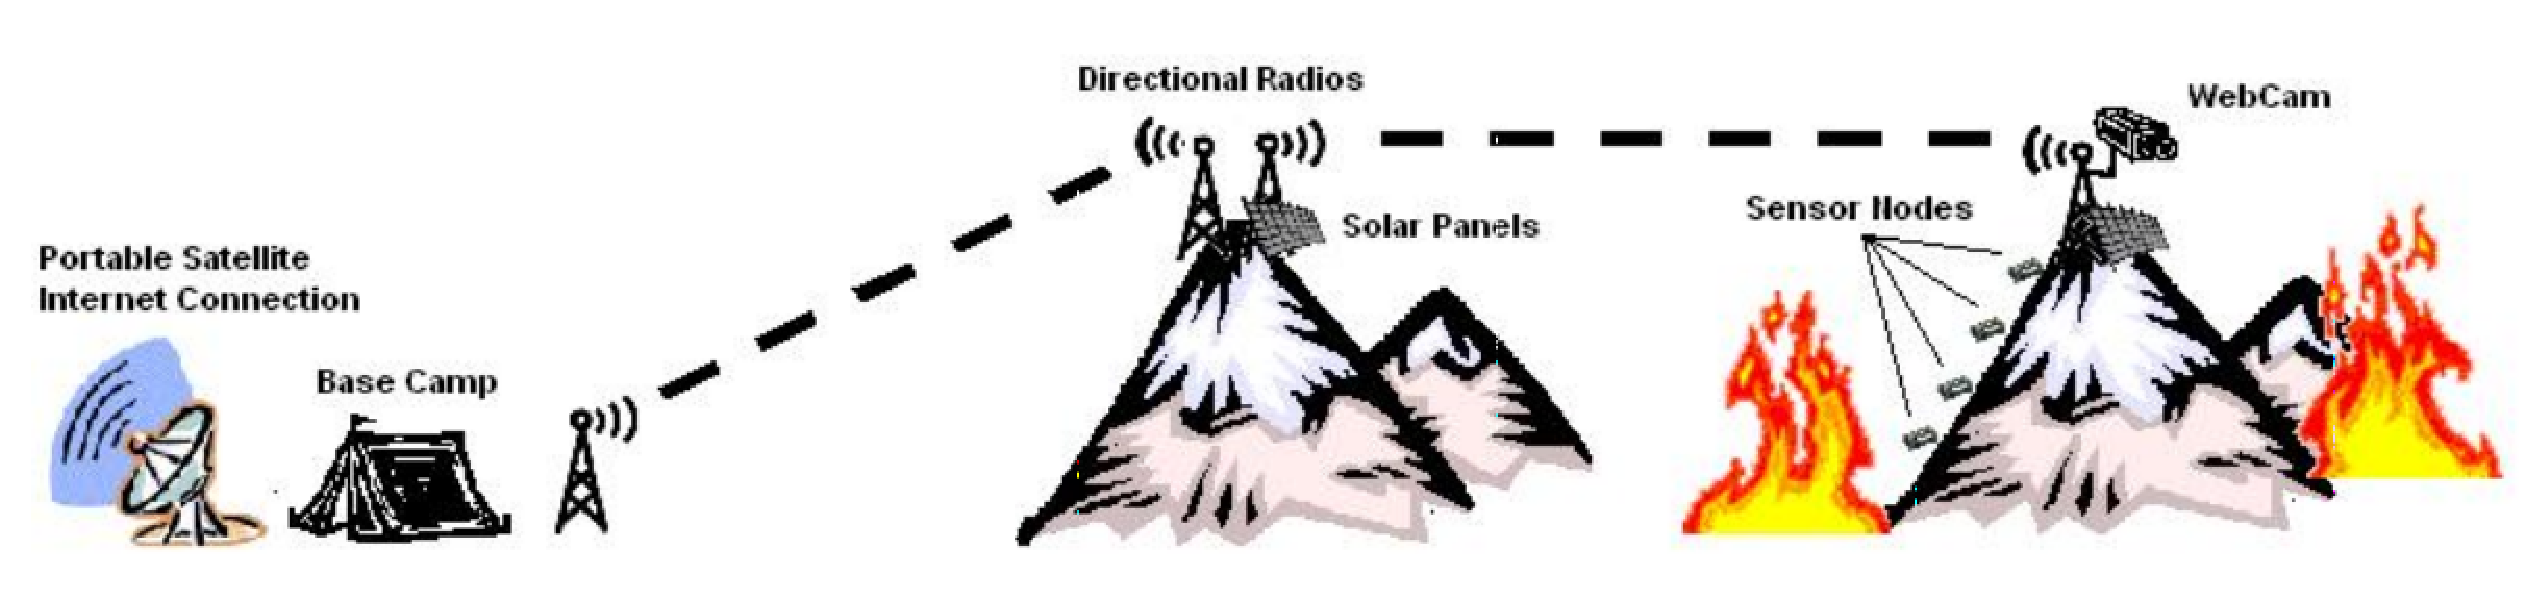
\includegraphics[width=140mm]{./images/firewxnet_overview.eps}
 \end{center}
 \caption{FireWxNet概要}
 \label{fig:firewxnet_overview}
\end{figure}


森林火災検知システムにおけるネットワークライフタイムは,
約6ヶ月から成る火災シーズンを少なくとも上回ることが望ましいが,
一般的にそれぞれのノードが数週間にわたって稼働することは難しいのが現状である.
したがってこの要件を満たすためにも,
エネルギーの消費を抑えるようなシステムを提案する必要がある.




\subsection{野生動物の生態調査}
%\vspace{0.5em}
生命科学における研究者たちは
動植物の観察時の
%人間という存在の潜在的影響について懸念を抱いていた.
人間が与える影響について懸念を抱いていた.
近年,無線センサネットワークが既存の動植物の観察手法に代わる
手法のひとつとして注目されている.
動物の場合一般的にセンサは繁殖期のはじまりに前もって設置され,
植物の場合にはセンサの設置は地面が凍る,もしくは休眠状態にあるときに設置されるため,
動植物に与える影響が少なく,
繰り返し現地調査を行うことが困難であるような危険な島におけるモニタリングへの
負担も軽減できることから,
無線センサネットワークを基盤としたモニタリングは,
センサネットワークが普及する以前の弊害を無視した手法と比較して,
目覚ましい業績をあげている.

%カリフォルニア大学バークレー校とインテルの研究員により,
%Mica Moteを基盤とした
%ウミツバメの生態を観測するための
%階層型センサネットワークがグレート・ダック島に展開された
%\cite{Mainwaring:2002:WSN:570738.570751}.
カリフォルニア大学バークレー校とインテルの研究員により
グレート・ダック島に展開された,
Mica Moteを基盤とした
ウミツバメの生態を観測するための
階層型センサネットワーク
\cite{Mainwaring:2002:WSN:570738.570751}
を生態調査の例として紹介する.
システム構成図は図\ref{fig:gdi_system_architecture}の通りである.
動物の掘った穴など,調査対象となる32箇所にMica Moteが設置され,
区画ごとにグループ化されたそれらのMoteは,
センサデータをゲートウェイまで転送し,
さらにローカルネットワークを通して,
ベースステーションまでデータを転送する.
その後,ベースステーションでデータを記録し,
定期的に複製されたデータはデータベースへと格納される.
ユーザはデータベースサーバ内の複製されたデータにアクセスすることや,
サンプリングレートや電力を操作する変数を調整するなどの,
インタラクションをするためのデバイスを利用することが可能である.

\begin{figure}[htbp]
 \begin{center}
  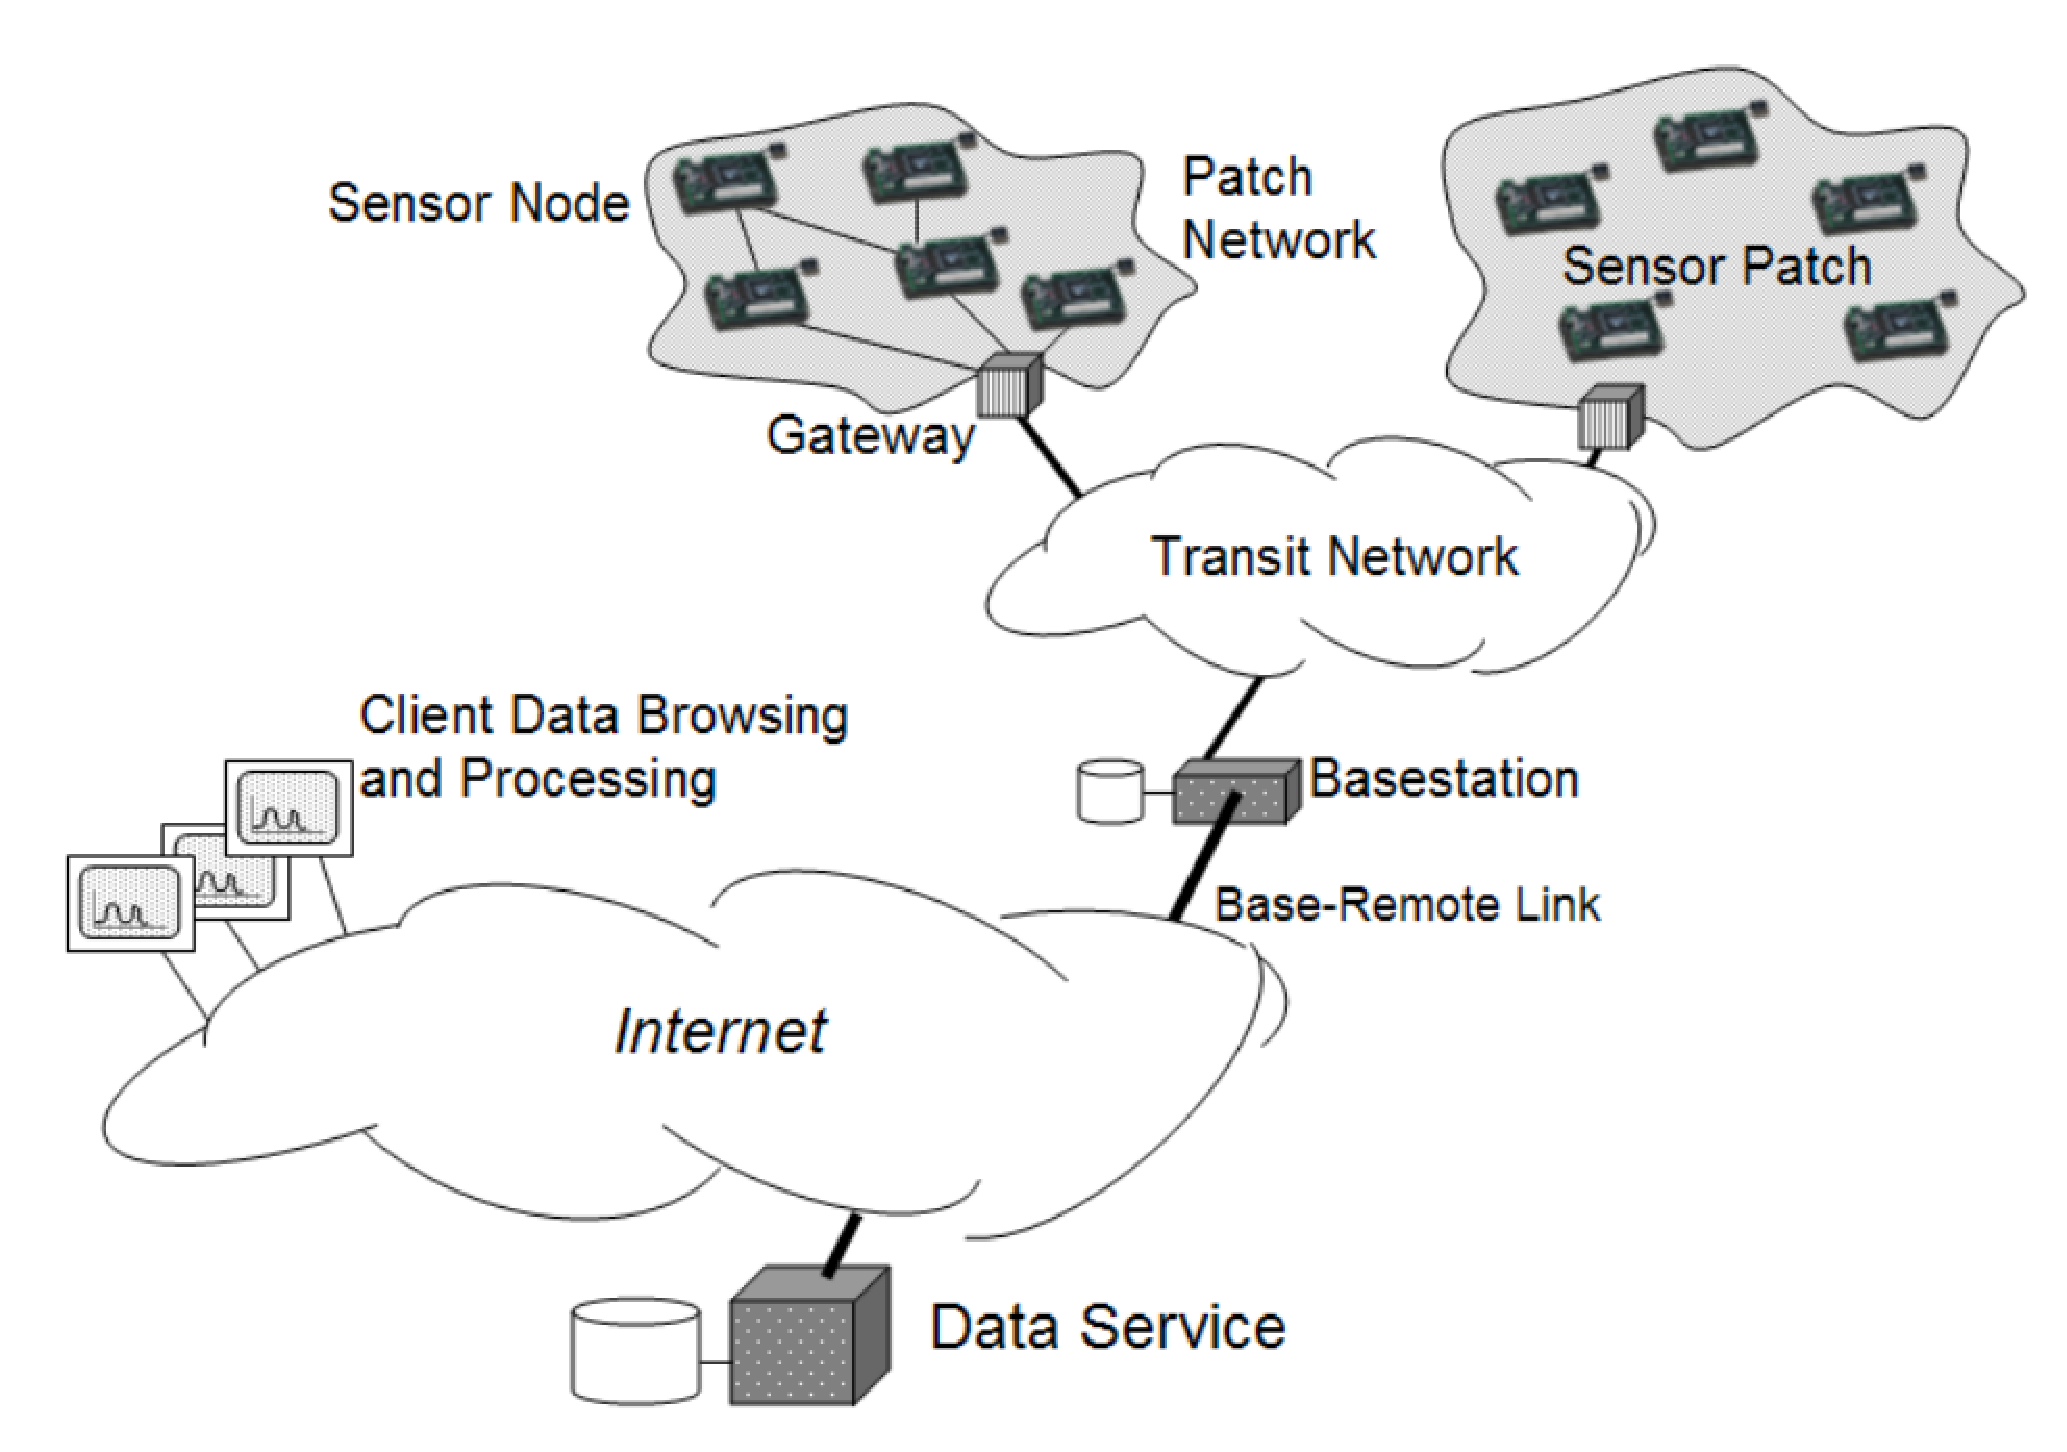
\includegraphics[width=120mm]{./images/gdi_system_architecture.eps}
 \end{center}
 \caption{GDIのシステム構成図}
 \label{fig:gdi_system_architecture}
\end{figure}


調査対象の特徴によっては,
現地調査を複数回行うことが困難となる場合があることは既に述べたが,
無線センサネットワークに用いられる小型デバイスにおける
バッテリの駆動時間は,一般的なラップトップなどと比較して
かなり短いのが現状である.
バッテリを交換する回数が増えるにつれ,
無線センサネットワークから得られる利益は減少してしまうため,
火災検知システムと同様に,省エネルギーが実現できるような
システム構成が求められている.




\section{ターゲットトラッキング}\label{sec:target_tracking}
%物理環境において,
特定のイベントの観測のための,
資源の限られた幾千ものセンサノードから成る
無線センサネットワーク技術に普及により,
様々なシナリオにおける無線センサネットワークの利活用が
現実的になりつつあることは既に述べたが,
交通量管理や侵入者検知などの
ターゲットトラッキングの分野も,
その影響が顕著に表れている分野のひとつである.

イベントを検知したセンサの周辺ノードはそのイベントを監視し,
ラップトップやベースステーションのような外界と通信する機能を持った
シンクノードに対してイベントの発生を知らせるのだが,
ターゲットトラッキングにおいて,
対象を検知し,その旨をシステムのゲートウェイノードに警告するタスクにより
中継されたデータは,
適時にゲートウェイまで届けられるべきである.
したがって,環境モニタリングと同様に
ターゲットトラッキングでもリアルタイムオペレーティングシステムを採用すべきである.
本節ではターゲットトラッキングの例として,
軍用監視システムについて言及する.


\subsection{軍用監視システム}
%\vspace{0.5em}
監視任務において,
ターゲットとする敵の能力や位置に関する情報を
正確に入手することが何よりも重要であるが,
そのような任務には隊員の危険を伴うものが多い.
無線センサネットワークを利用することで,
リスクを最小限に抑えつつ,
敵の侵入に関する情報を的確に把握する研究が盛んに行われている.
図\ref{fig:surveillance_system}は軍用監視システムにおける概念図である.

\begin{figure}[htbp]
 \begin{center}
  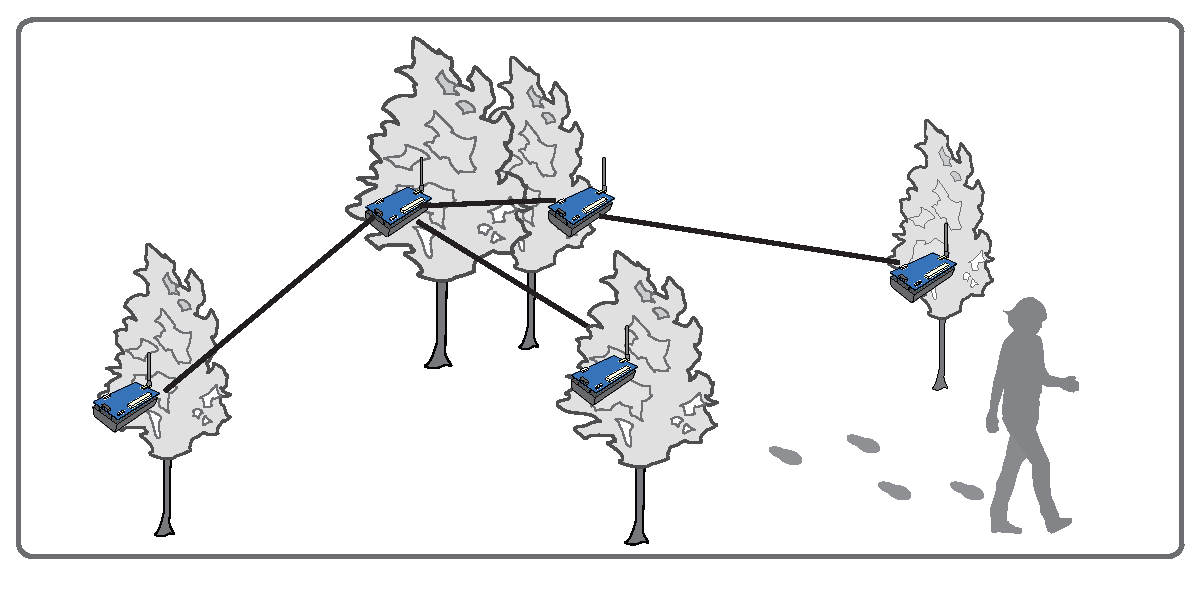
\includegraphics[width=100mm]{./images/surveillance_system.eps}
 \end{center}
 %\caption{イベント検知アプリケーション}
 %\caption{ターゲットトラッキングアプリケーション}
 \caption{軍用監視アプリケーションにおける概念図}
 \label{fig:surveillance_system}
\end{figure}


近年提案されている監視システムのほとんどが
シミュレーションを通して期待できる成果を挙げているが,
シミュレータを利用して単純化された仮説は
実環境において意図した通りの結果を得られないこともしばしばである.
Tian Heらの研究\cite{He04energy-efficientsurveillance}では,
省エネルギーかつステルス性を保ちながら移動する車両の位置を検知し,
追跡するセンサデバイスを用いた監視システムの設計と実装をし,
実空間においてシステムの感度を適宜調整することによって,
省エネルギー性と監視システムの性能におけるトレードオフについて考察している.
またこれに加えて,同期型の通信プロトコルを設計し,常にビーコンを送信し,
イベントが発生した場合はビーコンの送信を停止するProactive型と,
イベントが発生した場合にビーコンを送信するReactive型の実装を行い,
それぞれについて省電力性やステルス性などの評価も行っている.

監視システムアプリケーションを用いた任務は
数日から数ヶ月にかけて行われるものが一般的であり,
任務中の秘密保持の重大性や
任務が敵の管轄地域行われる場合もあることから,
%近づきにくさ
任務期間中に資源の制限されたセンサデバイスの手動による充電はできないことがほとんどである.
したがって任務期間中継続して使用するために,
監視システムにおけるアプリケーションでは
センサデバイスの寿命を向上させるような
省エネルギーな構成が必要とされる.

また軍用の監視システムにおいて,
デバイスが発見され,
それに伴った迎撃を
未然に防ぐことは極めて重要である.
センサデバイスを小型化することにより,
デバイスの発見を物理的に困難にすることができるが,
もしセンサデバイスが監視をする際に活発に通信をする場合,
無線周波数が傍受されてしまう可能性が高い.
重要なイベントが発生したときを除いて,
通信を控えることが求められている.


%今日,充電不可能なバッテリを用いた数ヶ月間稼働するセンサネットワークに対する
%関心が高まっている.



%\section{イベント検知アプリケーション}

\section{まとめ}
本章では,まず,技術の発展によりセンサノードの低価格化,高性能化が進み,
それに伴い,ネットワークに繋がる物理センサが自動的に多様なデータをやり取りし,
それらを様々な形で活用する無線センサネットワークが普及してきたことを説明した.
次いで,無線センサネットワークアプリケーションを
環境モニタリングとターゲットトラッキングに分類し,
それぞれについて例を紹介しながら
エネルギー節約とリアルタイム処理の重要性について言及した.


\chapter{無線センサネットワークにおけるオペレーティングシステム}
\begin{large}
\begin{quote}
本章では,最初にセンサネットワークの一般公衆化を説明し,公衆センサデータ管理における必須な機能要件である地理的探索について述べる.次に,公衆センサデータ管理のシステム設計の際の重要な概念であるデータ管理の時間的密度を解説し,最後にセンサデータの時間的特殊性とそれに起因する公衆センサデータ管理の問題点を述べる.
%本章では,
\end{quote}
\end{large}
\clearpage


%\section{無線センサネットワークにおけるオペレーティングシステム}
%無線センサネットワークのオペレーティングシステムには主に2種類あり,
%イベントモデルとスレッドモデルが存在している.
%無線センサネットワーク用のオペレーティングシステムではイベントモデルが主流となっている.

\section{イベントモデル}
イベントモデルで構築されたオペレーティングシステムは全てのタスクをイベントによって起動し,
run-to-completion で実行する形態のオペレーティングシステムである.
イベントモデルは図\ref{fig:event_model}に示されるように,
ひとつのイベントループと多数のイベントハンドラから構成される.
イベントループはイベントの到着を待ち,
イベントが届くとイベントに関連付けられているイベントハンドラを実行する.
イベントモデルではイベント駆動型プログラミングによってアプリケーションが記述される.
イベントハンドラは寿命の短いrun-to-completionで記述され,
プリエンプションされることがない.
つまり,イベントモデルはタスクは関数呼び出しと等価であり,
実行ストリームがひとつで実現されるため各タスクでローカル変数の領域を共有可能であることから,
省資源かつ低オーバヘッドで並列性を実現できる.
また,各タスクが不可分に実行されるので共有資源に対する排他制御が不要となり,
安全性が高い.
さらに,CPU の特殊な機能を用いなくても実装できるので移植性も高い.
\begin{figure}[htbp]
 \begin{center}
  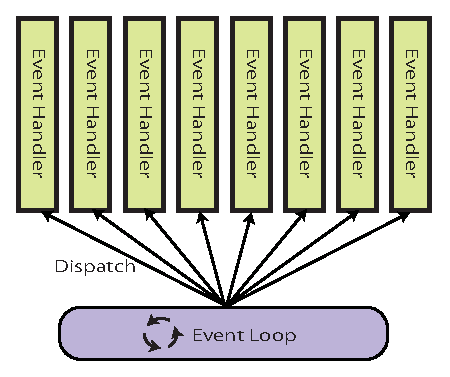
\includegraphics[width=60mm]{./images/event_model.eps}
 \end{center}
 \caption{イベントモデル}
 \label{fig:event_model}
\end{figure}


%\subsection{TinyOS: An Operating System for Sensor Networks}
\subsection{TinyOS}
イベント駆動型のオペレーティングシステムの中でも、最も代表的なものが
TinyOS\cite{Hill:2000:SAD:356989.356998}\cite{Levis04tinyos:an}である.
TinyOSはカリフォルニア大学バークレー校のSmartDust Projectで開発されたオペレーティングシステムである.
現在無線センサネットワークの標準的なオペレーティングシステムとして扱われており,
Crossbow社から発売されているMica2やMicaZ\cite{Hill:2002:MWP:623308.624560},
Telos\cite{Polastre:2005:TEU:1147685.1147744},iMote\cite{Nachman:2005:IMP:1147685.1147760}上で動作する.
TinyOSはCPUの特別な機能を使用せずに実装可能であるため,移植性が高く,
ATMELのAVR128LやTexsusのMSP430,ARM7などさまざまなCPUに移植されている.
TinyOSのアーキテクチャを図\ref{fig:system_conf_of_tinyos}に示す.

\begin{figure}[htbp]
 \begin{center}
  \includegraphics[width=100mm]{./images/system_conf_of_tinyos.eps}
 \end{center}
 \caption{TinyOS アーキテクチャ}
 \label{fig:system_conf_of_tinyos}
\end{figure}

TinyOSではnesC\cite{Gay:2003:NLH:781131.781133}と呼ばれるイベント駆動型の新しい言語で
複数のイベントハンドラを1つのモジュールとして設計可能な機能を提供している.
%TODO イラストレーターでnesCのコンパイルの様子を描く
図にnesC言語がコンパイルされて実行されるまでの流れを示す.
nesC言語はnesCコンパイラによってC言語のコードに変換された後,
Cコンパイラによって実行形式へと変換される.
nesC言語を採用することによって,
イベントモデルの持つプログラムの開発のし辛さを提供し,
新しい言語を学ばなければならないという手間がかかってしまうものの,
nesCはイベント駆動型に特化した最適化を行っているため省資源性を実現している.


%Earlier versions of TinyOS supported 
%a non-preemptive First-In-First-Out (FIFO) scheduling algorithm.
%Therefore, those versions of TinyOS do not support real-time application. 
%The core of the TinyOS execution model are tasks that run to completion in a FIFO manner.
%Since TinyOS supports only non preemptive scheduling, 
%task must obey run to completion semantics. 
%Tasks run to completion with respect to other task 
%but they are not atomic with respect to interrupt handlers, commands, and 
%events they invoke. 
%Since TinyOS uses FIFO scheduling, 
%disadvantages associated with FIFO scheduling are also associated with the TinyOS scheduler. 
%The wait time for a task depends on the task’s arrival time. 
%FIFO scheduling can be unfair to latter tasks especially 
%when short tasks are waiting behind longer ones.
%In [3], the authors claim that they have added support 
%for an Earliest Deadline First (EDF) scheduling algorithm in TinyOS, 
%to facilitate real-time applications. 
%The EDF scheduling algorithm does not produce a feasible schedule 
%when tasks content for resources. 
%Thus, TinyOS does not provide a solid real-time scheduling algorithm 
%if different threads content for resources. 

%TinyOS does not provide any explicit support for real-time applications. 
%As we already discussed in the scheduling section above, 
%tasks in TinyOS observe run to completion semantics in a FIFO manner, 
%hence in its original form, 
%TinyOS is not a good choice for sensor networks that are being deployed 
%to monitor real-time phenomena. 
%An effort has been made to implement an Earliest Deadline First (EDF) 
%process scheduling algorithm 
%and it has been made available in newer versions of TinyOS. 
%However, it has been shown that the EDF algorithm cannot produce a feasible schedule 
%when tasks content for resources. 
%In the nutshell, TinyOS is not a strong choice for real-time applications. 
%TinyOS does not provide any specific MAC, network, or transport layers protocol implementations
%that support Quality of Service requirements of real-time multimedia streams. 
%At the MAC layer, TinyOS supports TDMA, 
%which can be fine-tuned depending upon the requirements of an application 
%to support multimedia traffic streams.



%\subsection{A Dynamic Operating System for Sensor Nodes}
%\subsection{SOS}
%TinyOSがモノリシックなシステムイメージを持っていたのに対し,
%SOS\cite{Han:2005:DOS:1067170.1067188}は
%イベント駆動型オペレーティングシステムに動的モジュールの機能を実現したものである.
%SOSではカーネルから動的モジュールをロードする時に関数の型チェックを行うことで
%関数の型違反に伴うバグを防ぐ仕組みを取り入れている.

\subsection{Contiki}
Contiki\cite{Dunkels:2004:CLF:1032658.1034117}はC言語で記述された
最も正統派のイベント駆動型オペレーティングシステムである.
Contikiでは動的モジュールを実現するために
ELF(Executable and Linkable Format)形式のファイルを
ロード可能な仕組みを提供している\cite{Dunkels06run-timedynamic}.
Contikiのアーキテクチャを図\ref{fig:system_conf_of_contiki}に示す.


%Contiki [18], is a lightweight open source OS written in C for WSN sensor nodes. Contiki is a 
%highly portable OS and it is build around an event-driven kernel. Contiki provides preemptive 
%multitasking that can be used at the individual process level. A typical Contiki configuration 
%consumes 2 kilobytes of RAM and 40 kilobytes of ROM. A full Contiki installation includes features 
%like: multitasking kernel, preemptive multithreading, proto-threads, TCP/IP networking, IPv6, a 
%Graphical User Interface, a web browser, a personal web server, a simple telnet client, a screensaver, 
%and virtual network computing. 

Contikiにおいて,イベント駆動型の利点を失わずにスレッド形式で
プログラムの書きやすさを実現したのがProtothreads\cite{Dunkels:2006:PSE:1182807.1182811}である.
Protothreadsではイベントハンドラの中でスレッド的に動作させたい部分を
PT\_BEGINとPT\_ENDで囲み,
PT\_WAIT\_UNTILで条件付きブロックを行うことで,
イベントハンドラ実行中でも他のタスクに切り換えることを可能にしている.
このProtothreadsについては,\ref{sec:protothreads}において詳細に述べる.


\begin{figure}[htbp]
 \begin{center}
  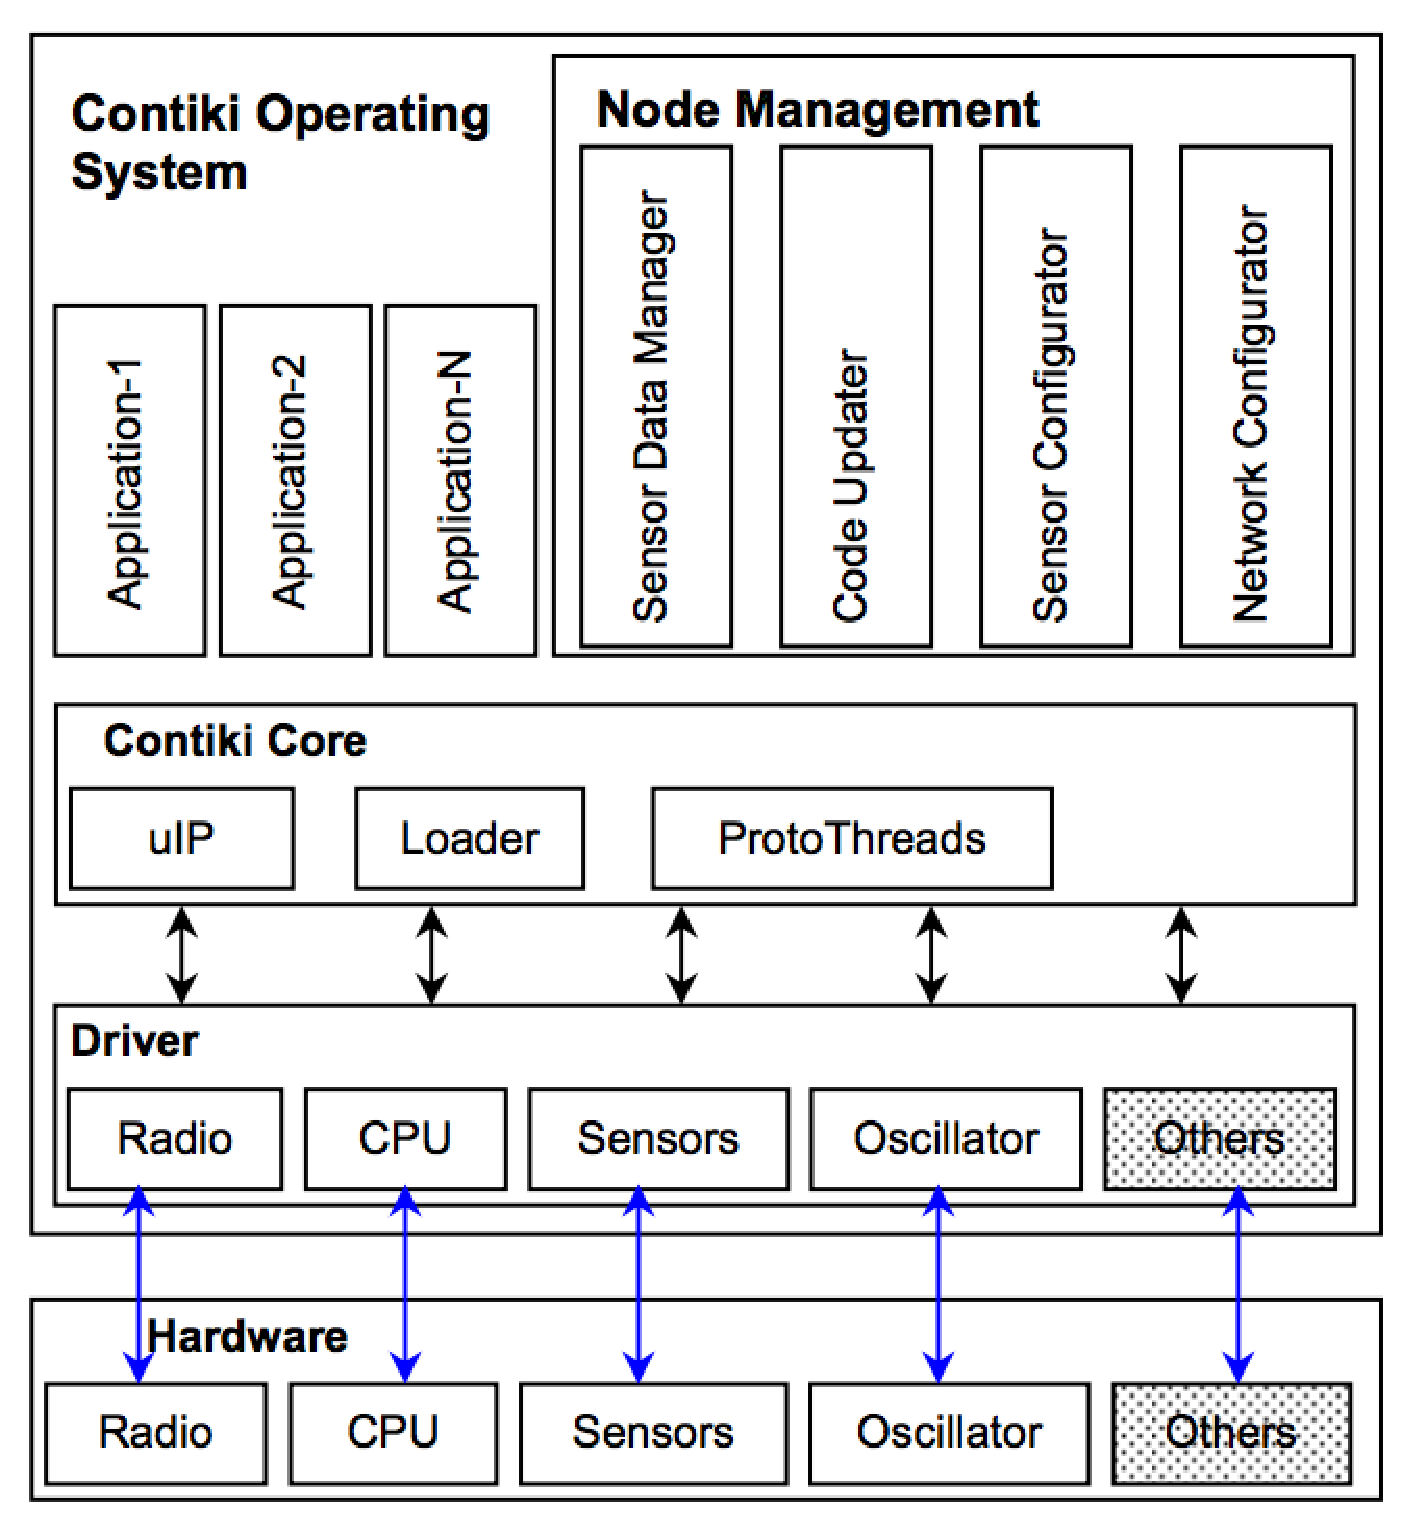
\includegraphics[width=80mm]{./images/system_conf_of_contiki.eps}
 \end{center}
 \caption{Contiki アーキテクチャ(参考:Operating Systems for Tiny Networked Sensors\cite{Dwivedi_operatingsystems})}
 \label{fig:system_conf_of_contiki}
\end{figure}




\section{スレッドモデル}
%スレッドモデルを図 5 に示す.
スレッドモデルは図\ref{fig:threads_model}に示されるように,
複数のスレッドから構成され,
各スレッドはそれぞれ独立に実行ストリームを持っており,
低い優先度のスレッドは高い優先度のスレッドにプリエンプションされるという特徴を持つ.
スレッドモデルではユーザはあたかもCPUを占有しているかのように
一連の処理をひとつのスレッドとして記述することができるため,
プログラムが書きやすい.
また,プリエンプションを行うことも想定しているため,
ハードリアルタイム処理をサポートすることができる.
\begin{figure}[htbp]
 \begin{center}
  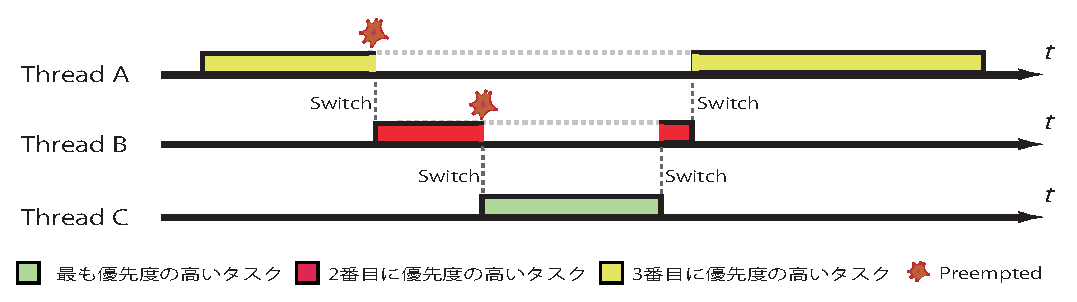
\includegraphics[width=140mm]{./images/threads_model.eps}
 \end{center}
 \caption{スレッドモデル}
 \label{fig:threads_model}
\end{figure}


%\subsection{Nano-RK: an Energy-aware Resource-centric RTOS for Sensor Networks}
\subsection{Nano-RK}
Nano-RK\cite{Eswaran:2005:NER:1106608.1106672}は,
無線センサネットワークにおけるマルチタスク処理機能を備えた
リアルタイムオペレーティングシステムであり,
%Nano-RK [31] is a fixed, preemptive multitasking real-time OS for WSNs. 
%Nano-RKを設計することで,
リソースの使用が制限された無線センサネットワークにおける,
マルチタスク処理,
優先度順位スケジューリングや
マルチホップネットワークのサポートを実現する.
%The design goals for Nano-RK are multitasking, support for multi-hop networking, 
%support for priority-based scheduling, 
%timeliness and schedulability, extended WSN lifetime, 
%application resource usage limits, and small footprint.
2KbのRAMと18KbのROMを使用し,
Rate Monotonic Scheduleingと
Rate Harmonized Scheduling\cite{Rowe:2008:RSS:1475690.1475895}を利用することによって,
ハードリアルタイムアプリケーションとソフトリアルタイムアプリケーションの
両方をサポートする.
%Nano-RK uses 2 Kb of RAM and 18 Kb of ROM. Nano-RK provides support for CPU, 
%sensors, and network bandwidth reservations.
%Nano-RK supports hard and soft real-time applications 
%by the means of different real-time scheduling algorithms, 
%e.g., rate monotonic scheduling and rate harmonized scheduling [32]. 
現在動作確認がとれているセンシングプラットフォームとして,
FireFly\cite{Rowe_firefly:a}と
MicaZ\cite{Hill:2002:MWP:623308.624560}が挙げられる.
Nano-RKのアーキテクチャは図\ref{fig:system_conf_of_nrk}のとおりである.
%Nano-RK provides networking support through socket-like abstraction. 
%Nano-RK supports FireFly [33] and MicaZ sensing platforms. 

\begin{figure}[htbp]
 \begin{center}
  \includegraphics[width=100mm]{./images/system_conf_of_nrk.eps}
 \end{center}
 \caption{Nano-RK アーキテクチャ}
 \label{fig:system_conf_of_nrk}
\end{figure}



%\subsection{MANTIS OS: An Embedded Multithreaded Operating System for Wireless Micro Sensor Platforms}
\subsection{MANTIS OS}
MANTIS OS\cite{Bhatti:2005:MOE:1160162.1160178}はLinuxやFreeBSDなどで
用いられているスレッドと同様の機能をセンサノード上で
実現したスレッドモデルのオペレーティングシステムである.
開発者はLinuxやFreeBSDなどで用いられているソフトウェアを
大きな変更無しにMANTIS OS上に移植することができる.
また,MANTIS OS上の1つのスレッドとして
TinyOS\cite{Hill:2000:SAD:356989.356998}\cite{Levis04tinyos:an}を
実装することも可能であり\cite{Trumpler06asystematic},
さまざまなソフトウェアリソースをMANTIS OS上で動作可能であることも特徴的である.
MANTIS OSはC言語で実装されており,
アプリケーション開発者もC言語を用いて開発を行うことが可能である.
図\ref{fig:system_conf_of_mantis}はMANTIS OSのアーキテクチャである.

%The MultimodAl system for NeTworks of In-situ wireless Sensors (MANTIS) provides 
%a new multithreaded operating system for WSNs.
%MANTIS is a lightweight and energy efficient operating system. 
%It has a footprint of 500 bytes, 
%which includes kernel, scheduler, and network stack. 
%The MANTIS Operating System (MOS) key feature is that 
%it is portable across multiple platforms, 
%i.e., we can test MOS applications on a PDA or a PC [28].
%Afterwards, the application can be ported to the sensor node.
%MOS also supports remote management of sensor nodes through dynamic programming. 
%MOS is written in C and it supports application development in C.
%The following subsections discuss the design features of MOS in more detail

\begin{figure}[htbp]
 \begin{center}
  \includegraphics[width=80mm]{./images/system_conf_of_mantis.eps}
 \end{center}
 \caption{MANTIS OS アーキテクチャ}
 \label{fig:system_conf_of_mantis}
\end{figure}



\section{イベントモデルとスレッドモデルの比較}
表\ref{tab:merit_and_demerit}にイベントモデルとスレッドモデルにおける
メリットとデメリットを示す.
既に述べたように,
イベントモデルではプリエンプションされることを前提としていないため,
実行ストリームがひとつで実現され,
ローカル変数の領域がそれぞれのタスクで共有することができるようになることから,
省資源で低オーバヘッドなシステムを構築することが可能になる.
しかしながら,イベントモデルではユーザが一連の処理を細かい処理に分割しなければならないため,
アプリケーションの開発が困難になってしまい,
%アプリケーション開発時に開発者がプログラムを書き辛いという問題が発生する.
ハードリアルタイム処理のサポートもできない.
%さらに,イベントモデルではタスクのプリエンプションをしないことを前提に設計されているので
%ハードリアルタイム処理のサポートができない.


イベントモデルに対して,
スレッドモデルでは複数のスレッドがそれぞれ独立に実行ストリームを保持しているため,
プリエンプションを可能とする.
結果として,スレッドモデルではリアルタイム性をサポートすることができる.
また,それぞれの処理をひとつのスレッドとみなし記述をすることが可能となるため,
開発者がアプリケーションを開発することを容易にする.
しかしながら,プリエンプション時のオーバヘッドの大きいことや必要とされる資源が多いこと,
スレッド間の共有資源へのアクセス制御が必要となるために
安全性が損なわれるなどの欠点を兼ね備えている.


%本節で述べたとおり,
%
%イベント駆動モデルではタスクの中断をしないことを前提に設計されているため,
%現在のセンサネットワーク用のオペレーティングシステムでは
%省資源性かつ低オーバヘッドであることと,
%リアルタイム性のサポートはトレードオフの関係にある.



\begin{table}[htb]
  \centering
  \caption{オペレーティングシステムの比較}
  \begin{tabular}{|c||c|c|c|c|} \hline
    \backslashbox{}{} & \multicolumn{2}{|c|}{メリット} & \multicolumn{2}{|c|}{デメリット} \\ \hline \hline
    イベントモデル & 省資源 & 低オーバヘッド & リアルタイム性の非サポート & プログラムが記述しにくい \\ \hline
    スレッドモデル & \multicolumn{2}{|c|}{リアルタイム性のサポート} & 資源の消費が大きい & 高オーバヘッド \\ \hline
  \end{tabular}
  \label{tab:merit_and_demerit}
\end{table}



%\section{リアルタイムスケジューリング}
%ジョブの実行を設定された時間通りに作動させることをリアルタイム処理という.
%リアルタイム処理には主に
%ハードリアルタイム処理と
%ソフトリアルタイム処理,の2種類がある.
%
%
%\subsection{ハードリアルタイム処理}
%課せられた処理が期限内に終了しなかったとき,
%システム全体に致命的なダメージが生じてしまうリアルタイム処理のことを
%ハードリアルタイム処理という.
%したがって,期限内での終了が保証されなければならないシステムに用いられる.
%
%\subsection{ソフトリアルタイム処理}
%ソフトリアルタイム処理を行うシステムでは,
%期限内に処理が終了しなくてもシステム全体に致命的なダメージを与えることはない.
%ただし,処理自体の価値は終了期限とともに減少していく.



\section{まとめ}
%本章では,まず,センサネットワークの一般公衆化について述べた.次いで,公衆センサデータがを扱ったシステム設計をする際に,データ管理の時間的密度という要素を考慮すべきであることを示した.そして,センサデータが時間的特殊性を持った多次元データであることを述べ,また,それに起因するセンサデータ管理における問題を提起した.
%システムにおける地理的探索の必要性について記した.さらに,センサデータ以外のコンテンツを扱うシステムとセンサデータを扱うシステムの対比を行い,広域センサデータ管理システムにおけるデータ管理の時間的密度という概念を説明し,最後に,センサデータの時間的特殊性を取り上げた後,それに起因するセンサデータ管理におけるデータ管理の時間的密度の高さという問題を提起した.


イベント駆動モデルではタスクの中断をしないことを前提に設計されているため,
現在のセンサネットワーク用のオペレーティングシステムでは省資源性かつ低オーバヘッドであることと,
リアルタイム性のサポートはトレードオフの関係にある.







%\chapter{Contiki - a Lightweight and Flexible Operating System for Tiny Networked Sensors}
%\chapter{無線センサネットワークにおけるProtothreadsを用いたリアルタイムスケジューラ}
\chapter{問題提起}
\begin{large}
\begin{quote}
本章では,最初に,本研究が提案するT-Ringという公衆センサデータ管理システムにおける,時間概念の扱いと,それに伴った保存アルゴリズムの概念説明を行う.次に,集中管理とSynapseとのデータ管理の時間的密度と計算コストの比較を行う.詳細な設計については次章で解説する.

\end{quote}
\end{large}
\clearpage

\section{Protothreads}\label{sec:protothreads}
既に述べたように,イベント駆動型は組み込みシステムやセンサネットワークにおいて,
主流なオペレーティングシステムとなっている.
しかし,イベント駆動型はメモリのオーバヘッド低く維持できる一方で,
ユーザが一連の処理を細かい処理に分割しなければならないため,
プログラムが書き辛いという問題が発生する(Listing\ref{lst:non-protothreads}).
%TinyOSの例
Protothreads\cite{Dunkels:2006:PSE:1182807.1182811}は
イベント駆動型プログラムをマルチスレッド型のように
記述することができるため(Listing\ref{lst:using-protothreads}),
メモリのオーバヘッドを抑えつつ,
イベント駆動型の欠点を補うことが可能となる.
本節では,Protothreadsの機能について詳しく述べる.



\begin{lstlisting}[caption=Protothredsを使用せずに記述した場合, label={lst:non-protothreads}]
struct pt {
    unsigned short lc;
};


char example(struct pt *pt) { 
    char PT_YIELD_FLAG = 1;

    if(PT_YIELD_FLAG) { ; }

    switch((pt)->lc) {
        case 0:
            while(1) { 
                do {
                    (pt)->lc = __LINE__;

        case: __LINE__:
                        if( !(condition) ) { // counter != 1000
                            return PT_WAITING;
                        } 
                } while(0);

                printf("Threshold reached\n");
                counter = 0;
            } 
    }
    PT_YIELD_FLAG = 0;
    (pt)->lc = 0;

    return PT_ENDED;
}
\end{lstlisting}



\begin{lstlisting}[caption=Protothredsを使用した場合, label={lst:using-protothreads}]
#include"pt.h"


PT_THREAD(example(structpt*pt)){
    PT_BEGIN(pt);

    while(1) {
        PT_WAIT_UNTIL(pt, counter == 1000);
        printf("Threshold reached\n");
        counter = 0;
    }
    
    PT_END(pt); 
}
\end{lstlisting}




\subsection{メモリ}
マルチスレッド型のオペレーティングシステムでは,
図\ref{fig:threads_stack}のようにそれぞれのスレッドにそれぞれのスタックを必要とする.
しかし,メモリが制限されているセンサネットワークのようなシステムでは,
スタック用のメモリは静的に保持されなければならないため,
このメモリを他の目的で使用することはできない.
\begin{figure}[htbp]
 \begin{center}
  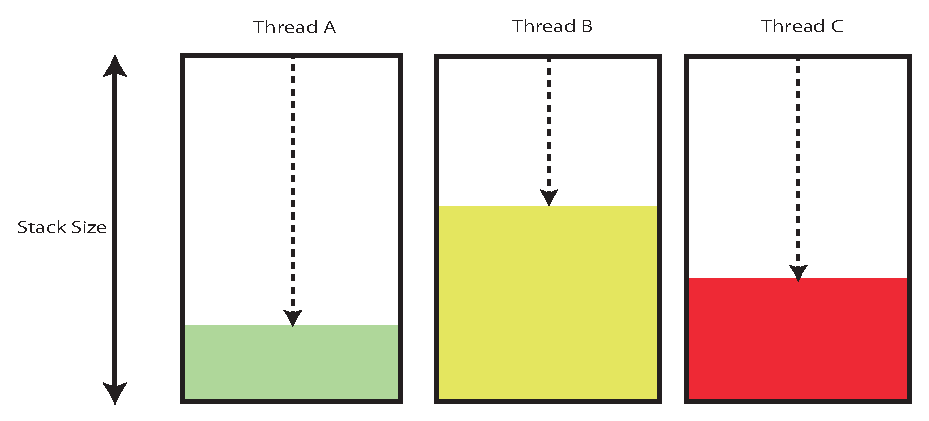
\includegraphics[width=110mm]{./images/threads_stack.eps}
 \end{center}
 \caption{一般的なスレッドモデルにおけるスタック}
 \label{fig:threads_stack}
\end{figure}

それに対して,Protothreadsにおけるスタックを図\ref{fig:protothreads_stack}に示す.
Protothreadsを使用した場合,
すべてのプログラムは同じスタックを共有し,
実行されることとなる.
つまり,Protothreadsを利用しているオペレーティングシステムではそのような事態を防ぐために,
マルチスレッドを実現しつつも,ひとつのスタックをあたかも複数個あるように見せかけている.
\begin{figure}[htbp]
 \begin{center}
  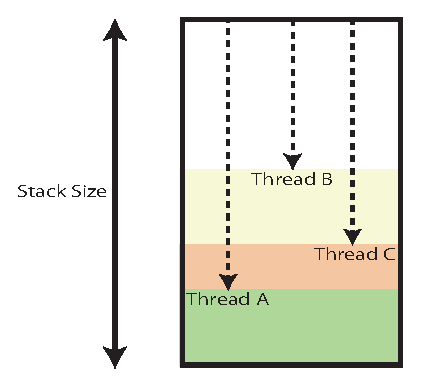
\includegraphics[width=45mm]{./images/protothreads_stack.eps}
 \end{center}
 \caption{Protothreadsにおけるスタック}
 \label{fig:protothreads_stack}
\end{figure}


\subsection{タスクの切り替え}
一般的なマルチスレッド型のオペレーティングシステムは,
タスクの割り込みがあった際には,
レジスタの状態を保存することで変数の値を保持し,
割り込まれたタスクの実行が終了したときに,
再びレジスタから変数を読み込み,
処理を途中から再開する.

しかし,Protothreadsを使用した場合,
状態をレジスタに保存することはせずに,
戻り値を利用することでタスクのCPUの利用を放棄する.
さらに,アプリケーション内の変数は静的な変数を採用しているため,
低オーバヘッドを実現しつつ,一貫性を保っている.

戻り値をもとにしたタスクの切り替えを行う際には,
スケジューラに対してプログラムのファイルの行数をreturnし,
各タスクがCPU利用権限を再度取得したとき,
行数を条件分岐し,前回中断した箇所から実行を
再開することとなる(Listing\ref{lst:using-protothreads}).

ただし,現在実行中のタスクよりも優先度の高いタスクが実行待ちになった際に,
他のマルチスレッドのオペレーティングシステムで実現されているように,
ループ内の処理を実行しているタスクに割り込みをし,
タスクを切り替えて実行することはできない.

現在では,タイマー割り込みを目的とした利用をされていない.
タイマーと現在時刻を比較し,
発火時刻を過ぎている場合,タスクを実行待ちのキューへと加える.
タイマーを実行するタスクは他のタスクと同じ優先度で周期的に実行される.




\subsection{イベント}
イベントモデルであるContikiでは,イベントが発生するとプロセスが実行される.
本節ではContikiで扱われる非同期イベントと同期イベントの違いについて説明する.

\subsubsection{非同期イベント}

\vspace{0.5em}非同期イベントが発生すると,
そのイベントはカーネルのイベントキューに挿入され,
実行時にFirst In First Outで呼び出される.

Asynchronous events are delivered to the receiving process some time after they have been posted.
Between their posting and their delivery, 
the asynchronous events are held on an event queue inside the Contiki kernel.

The events on the event queue are delivered to the receiving process by the kernel.
The kernel loops through the event queue and 
delivers the events to the processes on the queue by invoking the processes.



The receiver of an asynchronous event can either be a specific process, or all running processes.
When the receiver is a specific process, the kernel invokes this process to deliver the event.
When the receiver of an event is set to be all processes in the system,
the kernel sequentially delivers the same event to all processes, 
one after another.

非同期イベントはprocess\_post()関数によってポストされる.
process\_post()関数ははじめにキュー内にイベントのためのメモリ空間があるかどうかを決定するために,
現在のイベントキューのサイズを確認する.
もしメモリに空きがなければ,この関数はエラーを返し,
メモリに空きがあった際には,イベントをキューの最後に挿入する.

%Asynchronous events are posted with the process\_post() function. The internals of the process\_post() function is simple.
%It first checks the size of the current event queue to determine if there is room for the event on the queue.
%If not, the function returns an error.
%If there is room for the event on the queue,
%the function inserts the event at the end of the event queue and returns.

\begin{figure}[htbp]
 \begin{center}
  \includegraphics[width=115mm]{./images/fifo.eps}
 \end{center}
 \caption{非同期イベントの実行}
 \label{fig:asynchronous_event}
\end{figure}


\subsubsection{同期イベント}

\vspace{0.5em}When a synchronous event is posted,
the event is immediately delivered to the receiving process.

非同期イベントに対して,
同期イベントはポストされたとき,
同期イベント

Unlike asynchronous events, 
synchronous events are delivered directly when they are posted.
Synchronous events can only be posted to a specific processes.

同期イベントは即座に実行されるため,
同期イベントがポストされることは関数を呼び出すことに等しい.

Because synchronous events are delivered immediately,
posting a synchronous event is functionally equivalent to a function call: 
the process to which the event is delivered is directly invoked, 
and the process that posted the event is blocked until the receiving process has finished processing the event.
The receiving process is, however, not informed whether the event was posted synchronously or asynchronously.
\begin{figure}[htbp]
 \begin{center}
  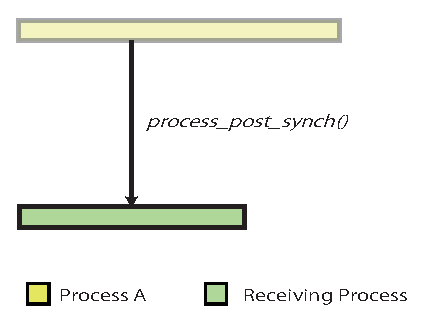
\includegraphics[width=40mm]{./images/synchronous_event.eps}
 \end{center}
 \caption{同期イベントの実行}
 \label{fig:synchronous_event}
\end{figure}


\subsubsection{ポーリング}

\vspace{0.5em}ポーリングリクエストはその他のイベントと異なる
ポールされたプロセスはprocess\_poll()関数によって呼び出され,
この関数がプロセス上で呼び出されるとそのプロセスは可能な限り早急にスケジューリングされる.

A poll request is a special type of event. A process is polled by calling the function process\_poll().
Calling this function on a process causes the process to be scheduled as quickly as possible.
The process is passed a special event that informs the process that it has been polled.

ポーリングはインタラプトからプロセスを実行する手法であり,
process\_poll()関数はプリエンプティブモードから安全に呼び出されるプロセスモジュールにおける,
唯一の関数である.

%Polling is the way to make a process run from an interrupt.
%The process\_poll() function is the only function in the process module that is safe to call from preemptive mode.

%\section{イベントタイマー}
%Contikiオペレーティングシステムには



\section{既存システムにおける問題意識}
イベント駆動モデルではタスクの中断をしないことを前提に設計されているため,
現在のセンサネットワーク用のオペレーティングシステムでは省資源性かつ低オーバヘッドであることと,
リアルタイム性のサポートはトレードオフの関係にある.
しかし,ターゲットトラッキングなどの状況においては,
通常時は省資源性かつ低オーバヘッドを実現し,
イベントが生じた際にはリアルタイム処理を行うことが必要となってくる.
それにも関わらず,現在双方を両立可能としたセンサネットワーク用のオペレーティングシステムは存在していない.

また,Protothreadsが
%イベント駆動型のオペレーティングシステムに実装されていながら,
マルチスレッド型のオペレーティングシステムとの親和性があると推測できることは既に述べたが,
既存のProtothreadsの実装ではイベントに優先度をつけることなく,
First In First Out(FIFO)の要領でイベントを呼び出している(図\ref{fig:asynchronous_event}).
本研究では環境モニタリングやターゲットトラッキングを想定環境としているため,
イベントの到着順でスケジューリングすることは好ましくない.
例えば,優先度の高いタスクが到着したときに既に多量のタスクが実行待ち状態となっている場合に,
高優先度のタスクが実行される頃には,既にそのタスクに実行する価値はない可能性がある.
したがって,既存手法とは別のアルゴリズムを用いてスケジューリングする必要がある.


%前述のとおり,一般的なマルチスレッド型のオペレーティングシステムでは,
%スレッド切り替え時にレジスタの状態を保存するのに対して,

Protothreadsでは,現在実行中のタスクよりも優先度の高いタスクが実行待ちになった際に,
他のマルチスレッドのオペレーティングシステムで実現されているように,
ループ内の処理を実行しているタスクに割り込みをし,
タスクを切り替えて実行することはできない.
これはタスクがreturnを発行するまでスケジューラが実行されないためである.


\section{本研究のアプローチ}


\section{まとめ}
本章では,まず,保存ピアの計算量を削減し,Synapseよりもデータ管理の時間的密度が高いアルゴリズムを提案することを述べた.次に,T-Ringにおいて時間という属性をDHTにおける保存ピアの決定における一つ要素としてではなく,保存ピアの変更を行うための要素として扱うことを述べた.そして,時間的密度,計算コストの観点から集中管理,Synapse,T-Ringの3つの手法の比較を行った.また,センサデータの時間的特殊性に着目した多次元センサデータ分散管理システムであるT-Ringの詳細な設計概念,設計実装について述べた.T-RingはP2Pのトポロジとして,代表的なアルゴリズムであるChordに準拠した1Dトーラスを用いている.保存ピアの参加や離脱なども同様にChordに準拠している.また,多次元データを扱うにあたり,Z-orderにより1次元化に言及した.時間的特殊性については,chunkとSPという2つの時間概念を導入し,保存ピア変更の基準とした.また,ユーザがT-Ringシステムを用いて,データ取得のクエリを送る際の,形式を定義した.




%\chapter{T-Ringの設計実装}
\chapter{設計と実装}
\begin{large}
\begin{quote}
%本章では,T-Ringにおける詳細な設計,実装について解説する.
本章では,本システムにおける機能要件,
概要,設計,さらに実装について説明する.
\end{quote}
\end{large}
\clearpage


\section{設計}

\subsection{機能要件}\label{sec:requirements}
ここでは本システムの設計にあたって,
\ref{sec:objective}で述べた本研究の目的を
達成するために必要となる機能について言及する.
%ここでは,\ref{sec:problems}で述べた既存研究における問題点を
%解決するという目的を達成するために必要となる機能について言及する.

\begin{enumerate}
\item{リアルタイム性}\\
時間的制約を伴ったタスクの処理が必要なアプリケーションを想定した場合,
オペレーティングシステムとして
リアルタイム処理を行えるものを選択すべきであり,
無線センサネットワークを用いた環境モニタリングでは,
%モニタリング対象の行動に変化があった際には,
イベント発生に応じてタスクを優先度を変化させる必要がある.
%このような時間的制約を伴ったタスクの処理が必要なアプリケーションを想定した場合,
%オペレーティングシステムとして
%リアルタイム処理を行うことが可能なものを選択することが多い.
また,ターゲットトラッキングにおいても同様に,
対象の検知は適時にゲートウェイまで届けられなければならない.
%イベントを検知したセンサの周辺ノードはそのイベントを監視し,
%ラップトップやベースステーションのような外界と通信する機能を持った
%シンクノードに対してイベントの発生を知らせるのだが,
%ターゲットトラッキングにおいて,
%対象を検知し,その旨をシステムのゲートウェイノードに警告するタスクにより
%中継されたデータは,
%適時にゲートウェイまで届けられるべきである.
%したがって,環境モニタリングと同様に
%ターゲットトラッキングでもリアルタイムオペレーティングシステムを採用すべきである.
\newline
\item{省資源性かつ低オーバヘッド}\\
森林火災検知システムにおけるネットワークライフタイムは,
火災シーズンを上回ることが望ましく,
%一般的にそれぞれのノードが数週間に渡って稼働することは難しいのが現状である.
%したがってこの要件を満たすためにも,
%エネルギーの消費を抑えるようなシステムを提案する必要がある.
野生動物の生態調査を行う際にも,
%調査対象の特徴によっては,
現地調査を複数回行うことが困難となる場合もあるため,
資源の限られたセンサノードにおいて低オーバヘッドを
維持することは極めて重要である.
%無線センサネットワークに用いられる小型デバイスにおける
%バッテリの駆動時間は,一般的なラップトップなどと比較して
%かなり短いのが現状である.
%バッテリを交換する回数が増えるにつれ,
%無線センサネットワークから得られる利益は減少してしまうことから,
%火災検知システムと同様に,省エネルギーが実現できるような
%システム構成が求められている.
監視システムアプリケーションを用いた任務でも,
%数日から数ヶ月にかけて行われるものが一般的であり,
%任務中の秘密保持の重大性や
%任務が敵の管轄地域行われる場合もあることから,
%近づきにくさ
任務期間中に資源の制限されたセンサデバイスの手動による充電はできないことがほとんどであることから,
同様の機能が必要であることが考えられる.
%したがって任務期間中継続して使用するために,
%監視システムにおけるアプリケーションでは
%センサデバイスの寿命を向上させるような
%省エネルギーな構成が必要とされる.
\end{enumerate}



\subsection{システム概要}
%本研究では,Contikiにスケジューラを実装することで,
%省資源性かつ低オーバヘッドを実現する.
前述のとおり,Contikiはイベント駆動型であるため,
省資源でありつつ,オーバヘッドを低く維持することが可能である.
またContikiにおけるProtothreadsは,
マルチスレッド型のオペレーティングシステムのようにプログラムを記述できるため,
イベント駆動型の欠点であるプログラムの書き辛さを改善することができ,
Protothreadsとマルチスレッド型のオペレーティングシステムは関係が密であると推測できる.
%したがって,今回のアプローチとして,Protothreadsを採用する.
しかしながら,Protothreadsを使用した場合,
タスクの実行を中断させるプリエンプションができないため,
本システムでは適時処理が必要なイベントが発生した際には,
コンテキストを保存し,スレッドを切り替えることができるような
設計が必要となる.

本システムの全体像を図\ref{fig:system_overview}に示す.
本システムは,ひとつのイベントループと多数のイベントハンドラから構成される.
イベントループはイベントの到着を待ち,
イベントが届くとイベントに関連付けられているイベントハンドラを実行する.
しかしながら,通常のイベントモデルのオペレーティングシステムと異なり,
本システムではリアルタイム処理の必要なイベントが発生する場合を想定している.
イベントループ実行中に,リアルタイムイベントが発生した場合には,
現在実行中のタスクをプリエンプションし,
スレッドを切り替え,リアルタイムタスク実行後再びイベントループの実行を再開する.
%スレッドモデルは図\ref{fig:threads_model}に示されるように,
%複数のスレッドから構成され,
%各スレッドはそれぞれ独立に実行ストリームを持っており,
%低い優先度のスレッドは高い優先度のスレッドにプリエンプションされるという特徴を持つ.





%イベントモデルではイベント駆動型プログラミングによってアプリケーションが記述される.
%イベントハンドラは寿命の短いrun-to-completionで記述され,
%プリエンプションされることがない.
%つまり,イベントモデルはタスクは関数呼び出しと等価であり,
%実行ストリームがひとつで実現されるため各タスクでローカル変数の領域を共有可能であることから,
%省資源かつ低オーバヘッドで並列性を実現できる.





%イベントモデルで構築されたオペレーティングシステムは全てのタスクをイベントによって起動し,
%run-to-completion で実行する形態のオペレーティングシステムである.
%イベントモデルは図\ref{fig:event_model}に示されるように,
%ひとつのイベントループと多数のイベントハンドラから構成される.
%イベントループはイベントの到着を待ち,
%イベントが届くとイベントに関連付けられているイベントハンドラを実行する.
%イベントモデルではイベント駆動型プログラミングによってアプリケーションが記述される.
%イベントハンドラは寿命の短いrun-to-completionで記述され,
%プリエンプションされることがない.
%つまり,イベントモデルはタスクは関数呼び出しと等価であり,
%実行ストリームがひとつで実現されるため各タスクでローカル変数の領域を共有可能であることから,
%省資源かつ低オーバヘッドで並列性を実現できる.
%また,各タスクが不可分に実行されるので共有資源に対する排他制御が不要となり,
%安全性が高い.
%さらに,CPU の特殊な機能を用いなくても実装できるので移植性も高い.
%本節では,TinyOSとContikiをイベントモデルの例として提示し,
%それぞれの特徴について言及する.


%スレッドモデルは図\ref{fig:threads_model}に示されるように,
%複数のスレッドから構成され,
%各スレッドはそれぞれ独立に実行ストリームを持っており,
%低い優先度のスレッドは高い優先度のスレッドにプリエンプションされるという特徴を持つ.
%スレッドモデルではユーザはあたかもCPUを占有しているかのように
%一連の処理をひとつのスレッドとして記述することができるため,
%プログラムが書きやすい.
%また,プリエンプションを行うことも想定しているため,
%%ジョブの実行を設定された時間通りに作動させる,
%ハードリアルタイム処理をサポートすることができる.





\begin{figure}[htbp]
 \begin{center}
  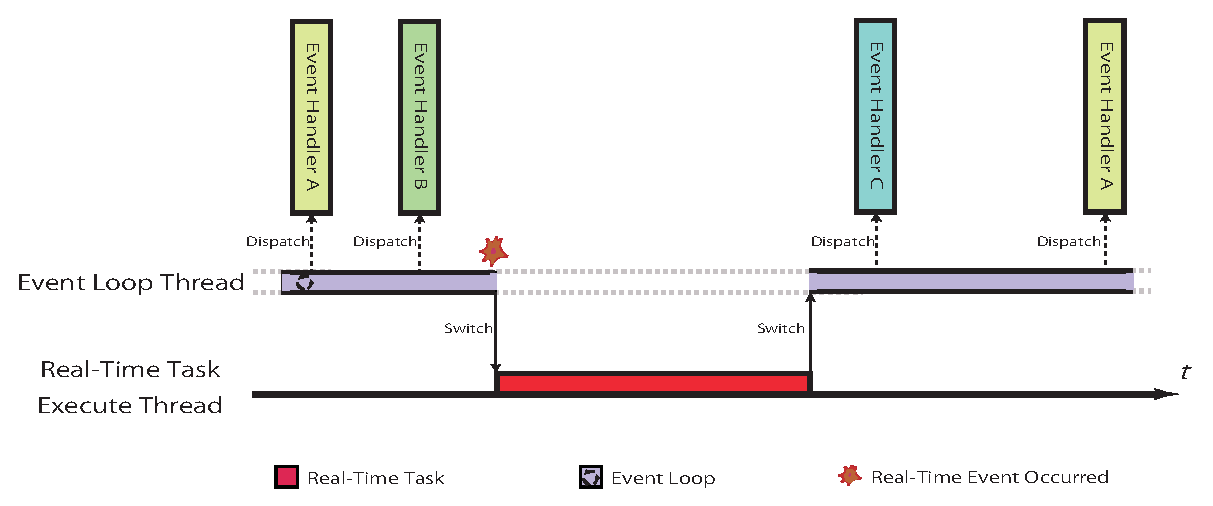
\includegraphics[width=150mm]{./images/system_overview.eps}
 \end{center}
 \caption{システム概要}
 \label{fig:system_overview}
\end{figure}


\subsection{システム構成}
%本節では,T-Ringシステムの設計について述べる.T-Ringを構成する保存ピアはネットワークモジュール,センサ情報管理モジュール,データ保存モジュール,データ取得モジュール,保存ピア発見モジュール,センサ管理モジュール,アプリケーションモジュールの7つのモジュールによって構成される.図\ref{fig:sysconf}がシステム構成図であり,各モジュール間でのデータの受け渡しが記述されている.
本節では,本システムのアーキテクチャ(図\ref{fig:system_architecture})を示し,
各モジュールについて詳しく説明する.


\begin{figure}[htbp]
 \begin{center}
  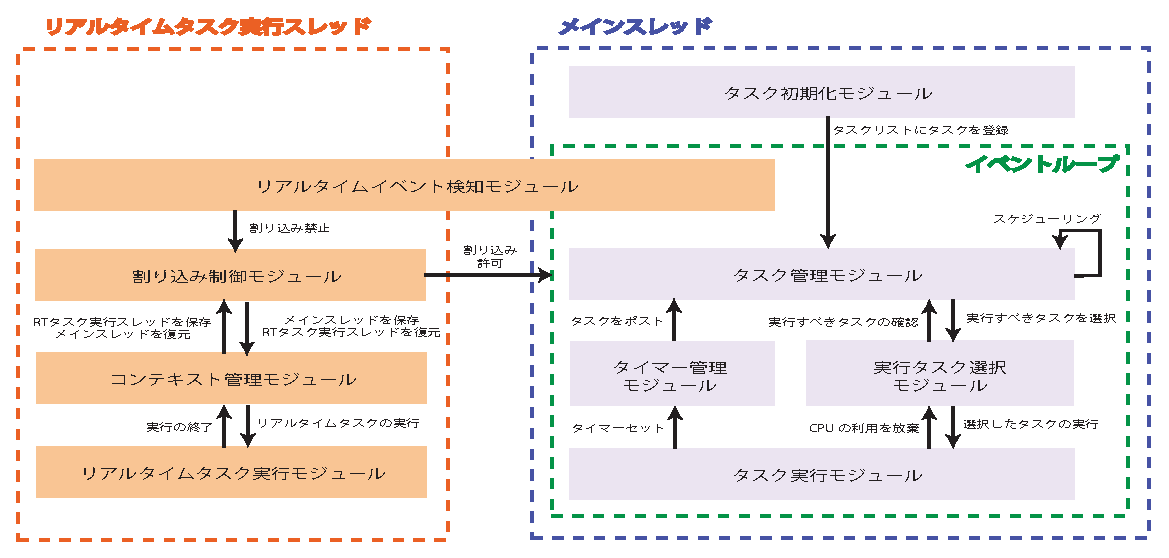
\includegraphics[width=150mm]{./images/system_architecture.eps}
 \end{center}
 \caption{システムアーキテクチャ}
 \label{fig:system_architecture}
\end{figure}


\subsubsection{タスク初期化モジュール}

\vspace{0.5em}タスク初期化モジュールは,アプリケーション開発者によって
初期化されたタスクをカーネルが保持するタスクリストに登録する.
本モジュールはアプリケーションがデプロイされたときにのみ実行され,
イベントループ内で実行されるモジュールと異なり,
複数回実行されることはない.



\subsubsection{タスク管理モジュール}

\vspace{0.5em}ここではタスク初期化モジュールにて,
登録されたタスクをタスクリストに登録し,
スケジューリングアルゴリズムに従って,
タイマー管理モジュールによってポストされるタスクを
実行される順番に並び替える.
実行タスク選択モジュールからの問い合わせがあった際には,
スケジューリング後の最も優先度の高いタスクのアドレスを渡す.



\subsubsection{実行タスク選択モジュール}

\vspace{0.5em}タスク実行モジュールにおいて,
実行中のタスクがCPUの利用を放棄した場合,
実行タスク選択モジュールにて,
次に実行するタスクを選択するために,
タスク管理モジュールに実行が最優先とされるタスクについて尋ねる.
タスク管理モジュールからの応答を待ち,
受け取ったタスクを次に実行するべく,
タスク実行モジュールへと引き渡す.



\subsubsection{タスク実行モジュール}

\vspace{0.5em}タスク実行モジュールでは,
タスク選択モジュールにて選択されたタスクを実行する.
実行中のタスクがCPUの利用を放棄した場合には,
次に実行するタイミングを決めるために,
タイマー管理モジュールに次の実行時間を知らせ,
タスク選択モジュールによって選ばれた
次に優先度の高いタスクを実行する.



\subsubsection{タイマー管理モジュール}

\vspace{0.5em}実行中のタスクが自ら実行を中断した場合,
タスク実行モジュールにて次に実行される時間が指定される.
タイマー管理モジュールでは,
タスク実行モジュールによってセットされたタイマーが発火した際には,
それに対応するタスクをポストするため,
タスク管理モジュールにタスクのポストを知らせる.


\subsubsection{リアルタイムイベント検知モジュール}

\vspace{0.5em}本システムの想定環境である,
環境モニタリングやターゲットトラッキングのようなアプリケーションでは,
イベントが発生した際に,他のどのタスクよりも優先してそのタスクの
実行を行う必要がある.
本モジュールでは,対象とするイベントが発生した場合に,
イベントループに割り込みをし,
他のスレッドにスイッチした際に割り込みが発生しないよう,
割り込み制御モジュールにて割り込みを禁止するシグナルの送信を依頼する.


\subsubsection{割り込み制御モジュール}

\vspace{0.5em}割り込み制御モジュールでは,
リアルタイムタスク実行中に他のタスクによる
割り込み処理が発生しないように制御を行う.
リアルタイム処理が終了した際には,
イベントループ実行中のメインスレッドにタスクの完了を知らせ,
割り込みを許可する.


\subsubsection{コンテキスト管理モジュール}

\vspace{0.5em}タスクの実行中に割り込みが発生した場合,
割り込みが発生しなかったときと同様の処理が行われなければならないため,
レジスタの値をスタックに退避させる.
それに対して,割り込み発生により実行されるタスクは,
以前の状態を取り戻すべく,スタックからコンテキストを復元する.
リアルタイムタスクの処理が完了し次第,
メインスレッドのコンテキストを復元し,
割り込み制御モジュールに割り込みを許可するように求める.



\subsubsection{リアルタイムタスク実行モジュール}

\vspace{0.5em}本モジュールは,コンテキスト管理モジュールでの
中断されたタスクの復元が完了し次第,
リアルタイム処理の必要なタスクの実行を行う.
タスクの実行が完了すると,
その旨をコンテキスト管理モジュールに伝え,
割り込み発生前の状態を復元する.








%\subsection{スケジューリングアルゴリズム}




\section{実装}
\subsection{実装環境}
本システムはMicaZ上で実装した.
表\ref{tab:implementation_env}にMicaZ及びアプリケーション作成に
用いたコンパイラの詳細を示す.
開発する際に使用した言語はC言語である.
%開発言語としてC言語を使用した.


\begin{table}[htb]
  \centering
  \caption{実装環境}
  \begin{tabular}{|l||c|} \hline
  	項目	 & 環境 \\ \hline \hline
	CPU & Atmega128L \\ \hline
	Clock	& 7.37 MHz \\ \hline
	メモリ & 4 KB \\ \hline
	コンパイラ	& avr-gcc 4.5.3 \\ \hline
	無線チップ	& CC2420 \\ \hline
	オペレーティングシステム & Contiki 2.6 \\ \hline
	プラットフォーム & MicaZ \\ \hline
  \end{tabular}
  \label{tab:implementation_env}
\end{table}



\subsection{タスクの状態遷移}
本システムで実行されるタスクには
図\ref{fig:state_transition}のような4種類の状態があり,
関数呼び出しによって,それぞれのタスクの状態は遷移する.
ここではタスクの状態の変遷について説明する.

アプリケーションがシステムにデプロイされると,
process\_start関数が実行され,状態はPROCESS\_STATE\_NONEから,
PROCESS\_STATE\_RUNNINGへと変化する.
すべてのタスクはPROCESS\_STATE\_NONE状態から
PROCESS\_STATE\_RUNNINGへと切り換えられることで,
実行される準備が整えられる.
つまり,カーネルの保持するタスクリストに
登録されているタスクはすべて,PROCESS\_STATE\_RUNNING
状態で実行までの間待機することとなる.

タスクが実行される際には,call\_process関数により,
スケジューリングされたタスクリストの中から
最も優先度の高いタスクが実行され,
PROCESS\_STATE\_RUNNINGからPROCESS\_STATE\_CALLEDとなる.
PROCESS\_STATE\_CALLED状態のタスクは実行を終えると自らCPUの利用を放棄するため,
PROCESS\_STATE\_RUNNING状態に戻り,
次に優先度の高いタスクの状態をPROCESS\_STATE\_CALLEDへと変え,
そのタスクの実行を行う.

タスクが実行されている最中に,
リアルタイムタスクによる割り込みが発生した場合,
process\_suspendが実行され,
状態はPROCESS\_STATE\_SUSPENDEDへと遷移する.
再びタスクが再開されるとき,
process\_resumeによりPROCESS\_STATE\_CALLED状態に復帰し,
中断した処理の続きを行う.

タスクが終了されるとき,
exit\_process関数は対象とされるタスクの状態を
PROCESS\_STATE\_NONEに変更し,
状態の変わったタスクはタスクリストから消去される.



\begin{figure}[htbp]
 \begin{center}
  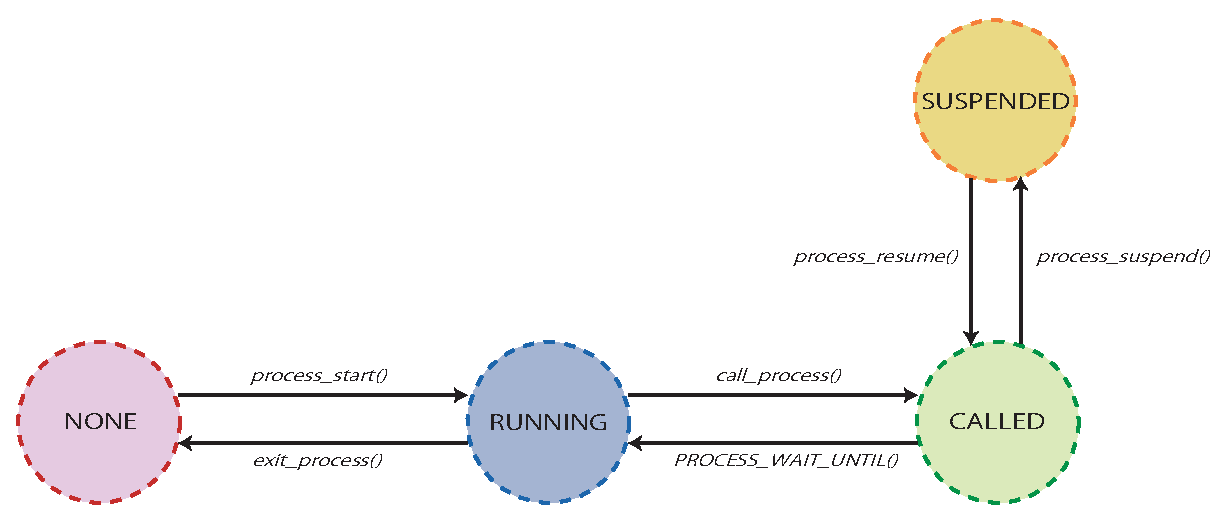
\includegraphics[width=130mm]{./images/state_transition.eps}
 \end{center}
 \caption{状態遷移図}
 \label{fig:state_transition}
\end{figure}




\section{まとめ}
本章では,
最初に本システムに必要な要件についてまとめ,
システムの概要について述べた.
そして,システムアーキテクチャを各モジュールに分解しながら説明し,
システム構成について考察した.
最後に実装環境など実装に関する内容について言及した.



%本章では,まず,ソフトウェアの構成について述べた,そして,個々のモジュールの細かな設計と実装について述べた.特に重要なアルゴリズムについては,各小節の末尾に実際のプログラムを掲載した.

\chapter{評価}
\begin{large}
\begin{quote}
本章では本システムの評価を行い,
結果について考察する.
\end{quote}
\end{large}
\clearpage

\section{評価方針}
本節では,本システムが
\ref{sec:requirements}で示した機能要件を満たしているかどうかを
実験を行うことで評価する.
具体的な方法について以下に述べる.


\begin{enumerate}
\item{リアルタイム性}\\
本研究は環境モニタリングやターゲットトラッキングのような
無線センサネットワークにおけるアプリケーションを対象としているため,
イベントモデルである拡張する前のContiki\cite{Dunkels:2004:CLF:1032658.1034117}
と本システムを比較し,
リアルタイムイベント発生から実行までの時間を評価する.
\newline
\item{消費電力}\\
本システムではリアルタイム処理が必要なイベントが発生しない場合には,
イベントモデルを採用している.
消費電力を抑えるという
要件が満たされているかどうかを確認するために,
%純粋なスレッドモデルであるNano-RK上で同様の動作をするアプリケーションを実行し,
%その際に消費される電力について評価を行う.
ランダムにリアルタイムイベントを発生させ,
イベント発生後現在の電圧をベースステーションへと送信する
アプリケーションを,
拡張前のContikiと本システム上で実行し,
それぞれの消費電力を比較し,考察する.
\end{enumerate}




%一般的なイベント駆動型のオペレーティングシステムでは,
%タスクは実行待ち状態になった順に実行されるため,
%重要なタスクが実行されず,
%そのタスク実行時にはその価値がなくなってしまうこともあるだろう.
%リアルタイム処理をサポートすれば,
%重要なタスクから順に処理を実行していくため,
%このように重要なタスクを未処理のまま終えてしまうような
%事態を未然に防ぐことができる.
%
%リアルタイム処理をサポートすることにより,
%低消費電力での運用も実現可能となる.
%リアルタイムタスクを効率的に処理可能なオペレーティングシステムと,
%効率の悪いオペレーティングシステムを比較した場合,
%前者の方が同じ精度のサービスを実現する場合に
%低いクロックで動作することができる.
%また,センサノード上では無線やセンサなどの
%周辺デバイスは必要のないときにスリープされることで消費電力を抑えている.
%このとき,リアルタイムタスクが処理可能ならば,
%素早く周辺デバイスのオンとオフを
%切り替えることができるようになるため,
%低消費電力を維持することが期待される.
%さらに,リアルタイム処理をサポートすることで,
%効率的に無線資源を利用し,
%無線通信に伴う電力を削減することができるだろう.



\section{リアルタイム性における評価}
\subsection{導入}
タスクの総数を一定にした場合と
タスクの総数を変化させる場合についてそれぞれ,
イベント発生の頻度を変化させながら,
リアルタイムイベントが発生してから
対象となるタスクが実行されるまでの時間(Latency)を評価する.
イベント発生の頻度を変化させるために,
Contikiにおけるイベントタイマーによってセットされる値を変化させる.
イベントタイマーは,
タイマーと現在時刻を比較し,
発火時刻をすぎている場合,
タスクをキューへと加える.
%タイマーを実行するタスクは他のタスクと同じ優先度で周期的に実行される.
%イベント発生の頻度に関しては,
%1秒あたりの
%システムクロックによって生成される一定のテンポ(tick)数を
%CLOCK\_CONF\_SECONDとし,
%イベント発生の時刻をこのCLOCK\_CONF\_SECONDを
%具体的に,基準となる値(CLOCK\_CONF\_SECOND)を用いて変化させていく.
また,システムの安定性を評価するために,
累積確率密度関数(Cumulative Distribution Function)
を評価に取り入れ,
その結果について\ref{sec:rt_discussion}にて考察する.



\subsection{評価環境}
本評価ではContikiのために設計された仮想マシン上の
シミュレータCooja\cite{osterlind2006cross}を利用する.
仮想マシンの詳細を表\ref{tab:instant_contiki}に記す.
また\ref{sec:implement_env}で示したように,
本実験では対象とするノードとしてMicaZ\cite{Hill:2002:MWP:623308.624560}
を利用する.
%を利用し,タスクの総数とイベント発生の頻度を変化させ,
%それぞれについてリアルタイムイベントが発生してから,
%対象となるタスクが実行されるまでの時間(Latency)を
%評価する.

\begin{table}[htbp]
  \centering
  \caption{評価環境}
  \begin{tabular}{|l||c|} \hline
  	項目	 & 環境 \\ \hline \hline
	オペレーティングシステム & Ubuntu 12.04 \\ \hline
	メモリ & 1024 MB \\ \hline
  \end{tabular}
  \label{tab:instant_contiki}
\end{table}


\subsection{実験結果}
%本評価項目における結果について示す.
%イベント発生の頻度に関しては,
%1秒あたりの
%システムクロックによって生成される一定のテンポ(tick)数を
%CLOCK\_CONF\_SECONDとし,
%イベント発生の時刻をこのCLOCK\_CONF\_SECONDを
タスクの総数を一定にした場合と
タスクの総数を変化させる場合についてそれぞれ,
%イベント発生の頻度を変化させながら,
実験によって得られた結果を示す.
以降より,Contikiは拡張前のContikiを,
D-Switchは拡張された後のContikiを示すこととする.

\subsubsection{タスクの総数を固定した場合}

\vspace{0.5em}タスクの総数を固定し,
実験ごとにイベントの発生頻度を増やしながら300秒ずつ,3回行った.

\begin{enumerate}
\item{実験1}\\
表\ref{tab:latency1},図\ref{fig:latency1}
からわかるように,
D-SwitchとContikiを比較してみると,
最小値,中央値の値に差異は見られない.
しかしながら,
ContikiにおけるLatencyの最大値が
163msを記録することが数回あったため,
平均値,標準偏差ともにD-Switchを上回る結果となった.
また図\ref{fig:cdf1}より,
Contikiでは最小値を記録した回数が
D-Switchよりも多いが,
D-SwitchではLatencyが81ms以下となる場合が
98\%を占めているため,
D-Switchの方が安定して低いLatencyを維持することに成功している.
\newline
\item{実験2}\\
表\ref{tab:latency2},図\ref{fig:latency2}より
実験1と同様にLatencyを比較したところ,
最小値,中央値の値に差異はなく,
最大値は実験1で得られた値に等しい.
しかしながら,
実験1と比較して,ContikiにおけるLatencyが最大となる
場合が多く,平均値,標準偏差の値が増加した.
図\ref{fig:cdf2}により得られた
累積密度確率関数の結果も
図\ref{fig:cdf1}と類似している.
\newline
\item{実験3}\\
表\ref{tab:latency3},図\ref{fig:latency3}が示すとおり,
最小値はContikiがD-Switchを下回ったが,
最大値はContikiがD-Switchを上回る245msを記録しているため,
ContikiにおけるLatencyの
平均値,標準偏差がそれぞれD-Switchを上回る結果となった.
%上記の実験と比較して,
%D-Switchは平均値,標準偏差ともに大きな変化は見られないが,
%実験2と比較したところ,
さらに図\ref{fig:cdf3}より,
D-Switchでは94\%が81msのLatencyでリアルタイムタスクの実行を
行うことができており,
安定性においてD-Switchの優位性を示している.
\end{enumerate}


\begin{table}[htbp]
  \centering
  \caption{実験結果1}
  \begin{tabular}{|c||c|c|c|c|c|} \hline
    \backslashbox{}{} & 最小値(ms) & 最大値(ms) & 中央値(ms) & 平均値(ms) & 標準偏差 \\ \hline \hline
    D-Switch & 80 & 82 & 81 & 81 & 0.17 \\ \hline
    Contiki & 80 & 163 & 81 & 97.97 & 33.39 \\ \hline
  \end{tabular}
  \label{tab:latency1}
\end{table}

\begin{figure}[htbp]
 \begin{center}
  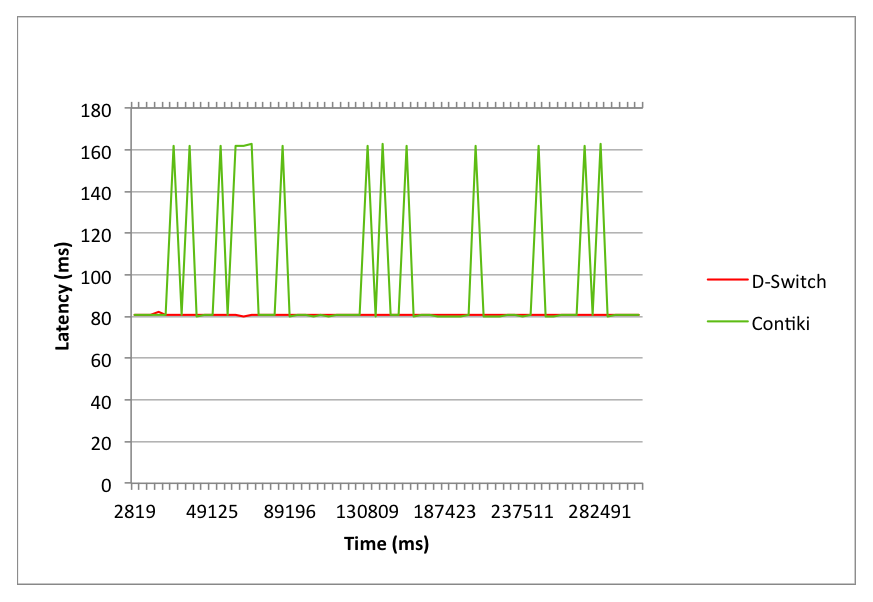
\includegraphics[width=120mm]{./images/latency1.eps}
 \end{center}
 \caption{Latency1}
 \label{fig:latency1}
\end{figure}

\begin{figure}[htbp]
 \begin{center}
  \includegraphics[width=120mm]{./images/cdf1.eps}
 \end{center}
 \caption{累積確率密度関数1}
 \label{fig:cdf1}
\end{figure}


\begin{table}[htbp]
  \centering
  \caption{実験結果2}
  \begin{tabular}{|c||c|c|c|c|c|} \hline
    \backslashbox{}{} & 最小値(ms) & 最大値(ms) & 中央値(ms) & 平均値(ms) & 標準偏差 \\ \hline \hline
    D-Switch & 80 & 82 & 81 & 81.02 & 0.19 \\ \hline
    Contiki & 80 & 163 & 81 & 108.37 & 38.49 \\ \hline
  \end{tabular}
  \label{tab:latency2}
\end{table}

\begin{figure}[htbp]
 \begin{center}
  \includegraphics[width=120mm]{./images/latency2.eps}
 \end{center}
 \caption{Latency2}
 \label{fig:latency2}
\end{figure}

\begin{figure}[htbp]
 \begin{center}
  \includegraphics[width=120mm]{./images/cdf2.eps}
 \end{center}
 \caption{累積確率密度関数2}
 \label{fig:cdf2}
\end{figure}


\begin{table}[htbp]
  \centering
  \caption{実験結果3}
  \begin{tabular}{|c||c|c|c|c|c|} \hline
    \backslashbox{}{} & 最小値(ms) & 最大値(ms) & 中央値(ms) & 平均値(ms) & 標準偏差 \\ \hline \hline
    D-Switch & 81 & 82 & 81 & 81.02 & 0.24 \\ \hline
    Contiki & 80 & 245 & 81 & 98.36 & 49.61 \\ \hline
  \end{tabular}
  \label{tab:latency3}
\end{table}

\begin{figure}[htbp]
 \begin{center}
  \includegraphics[width=120mm]{./images/latency3.eps}
 \end{center}
 \caption{Latency3}
 \label{fig:latency3}
\end{figure}

\begin{figure}[htbp]
 \begin{center}
  \includegraphics[width=120mm]{./images/cdf3.eps}
 \end{center}
 \caption{累積確率密度関数3}
 \label{fig:cdf3}
\end{figure}



\subsubsection{タスクの総数を変化させた場合}

\vspace{0.5em}タスクの総数を増やしながら
実験を300秒ずつ,2回行った.

\begin{enumerate}
\item{実験4}\\
表\ref{tab:latency4},図\ref{fig:latency4}が示すとおり,
ContikiではLatencyの最小値が80msを記録し,
両者における最小値となったが,
D-Switchでは観測されたすべての値が81msを記録しており,
標準偏差0を示したことや,
100\%が81msのLatencyで実行されていること
(図\ref{fig:cdf4})からも,
本システムの安定性を裏付ける結果となった.
\newline
\item{実験5}\\
表\ref{tab:latency5},図\ref{fig:latency5}より,
Contikiにおける最大値,平均値,標準偏差は
全実験中最大の値となった.
それに対して,D-Switchは
図\ref{fig:cdf5}にも示されるように,
97\%が81ms以内にリアルタイムタスクの実行を許可されている.
\end{enumerate}



\begin{table}[htbp]
  \centering
  \caption{実験結果4}
  \begin{tabular}{|c||c|c|c|c|c|} \hline
    \backslashbox{}{} & 最小値(ms) & 最大値(ms) & 中央値(ms) & 平均値(ms) & 標準偏差 \\ \hline \hline
    D-Switch & 81 & 81 & 81 & 81 & 0 \\ \hline
    Contiki & 80 & 326 & 81 & 102 & 48.52 \\ \hline
  \end{tabular}
  \label{tab:latency4}
\end{table}

\begin{figure}[htbp]
 \begin{center}
  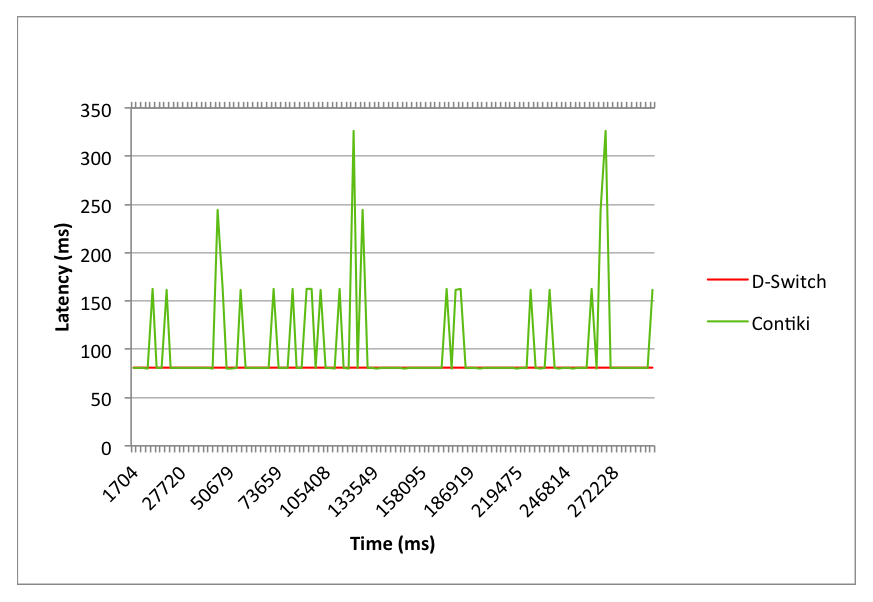
\includegraphics[width=120mm]{./images/latency4.eps}
 \end{center}
 \caption{Latency4}
 \label{fig:latency4}
\end{figure}

\begin{figure}[htbp]
 \begin{center}
  \includegraphics[width=120mm]{./images/cdf4.eps}
 \end{center}
 \caption{累積確率密度関数4}
 \label{fig:cdf4}
\end{figure}



\begin{table}[htbp]
  \centering
  \caption{実験結果5}
  \begin{tabular}{|c||c|c|c|c|c|} \hline
    \backslashbox{}{} & 最小値(ms) & 最大値(ms) & 中央値(ms) & 平均値(ms) & 標準偏差 \\ \hline \hline
    D-Switch & 80 & 82 & 81 & 81.02 & 0.21 \\ \hline
    Contiki & 80 & 327 & 81 & 121.26 & 63.95 \\ \hline
  \end{tabular}
  \label{tab:latency5}
\end{table}

\begin{figure}[htbp]
 \begin{center}
  \includegraphics[width=120mm]{./images/latency5.eps}
 \end{center}
 \caption{Latency5}
 \label{fig:latency5}
\end{figure}

\begin{figure}[htbp]
 \begin{center}
  \includegraphics[width=120mm]{./images/cdf5.eps}
 \end{center}
 \caption{累積確率密度関数5}
 \label{fig:cdf5}
\end{figure}

\subsection{考察}\label{sec:rt_discussion}
%ここでは,リアルタイムイベントが発生してから
%タスクが実行されるまでの時間について考察を行う.
図\ref{fig:d-switch_latency},
図\ref{fig:contiki_latency}はそれぞれ,
D-Switch,ContikiのLatencyに関するすべての実験結果を,
図\ref{fig:cdf_d-switch},
図\ref{fig:cdf_contiki}はそれぞれ,
D-Switch,Contikiの累積確率密度関数に関するすべての実験結果を示している.
実験1から実験3にてわかるようにイベントの発生頻度が
増加した場合,
ContikiではLatencyが増加することが伺える.
同様に実験4から実験5のようなタスクの総数が増加した場合にも,
ContikiにおけるLatencyは増加する傾向にある.

\ref{sec:asynchronous_event},\ref{sec:problems}
で示したように,
Contikiでは発生したイベントは
FIFOの要領でポストされていくため,
イベントが発生された際に
キューにすでに実行待ちのイベントが挿入されていた場合,
実行される時間が遅くなってしまう.
それに対して,
D-Switchでは,リアルタイムイベントが発行された際には,
実行中のタスクがあった場合でも,
そのタスクの実行を一時中断して,
リアルタイムタスクの実行を行うことができるため,
Latencyを低く維持することを可能にしている.

D-SwitchにおけるLatencyが80msに収束しているのは,
イベント発生から現在のコンテキストを保存するまでの時間だと推測される.
それに対して,Contikiには実行中のタスクをプリエンプションしてリアルタイムタスクを
行うことができないため,
リアルタイムイベントが発生した場合でも,
実行中のタスクの終了を待たなければならない.
ContikiにおけるLatencyの最小値が80msとなっているのは,
リアルタイムタスクが発生してから,
前のタスクの実行が終了するまでの時間であると考えられる.


\begin{figure}[htbp]
 \begin{minipage}{0.5\hsize} \begin{center}
     \includegraphics[width=70mm]{./images/d-switch_latency.eps}
    \end{center}
    \caption{D-Switch Latency}
    \label{fig:d-switch_latency}
 \end{minipage}
 \begin{minipage}{0.5\hsize}
    \begin{center}
     \includegraphics[width=70mm]{./images/contiki_latency.eps}
    \end{center}
    \caption{Contiki Latency}
    \label{fig:contiki_latency}
 \end{minipage}
\end{figure}




\begin{figure}[htbp]
 \begin{minipage}{0.5\hsize} \begin{center}
     \includegraphics[width=70mm]{./images/cdf_d-switch.eps}
    \end{center}
    \caption{D-Switch 累積確率密度関数}
    \label{fig:cdf_d-switch}
 \end{minipage}
 \begin{minipage}{0.5\hsize}
    \begin{center}
     \includegraphics[width=70mm]{./images/cdf_contiki.eps}
    \end{center}
    \caption{Contiki 累積確率密度関数}
    \label{fig:cdf_contiki}
 \end{minipage}
\end{figure}




\section{消費電力における評価}

\subsection{評価環境}
%消費電力に関する評価を行う際に,
実機のMicaZを使用して,
ランダムにリアルタイムイベントを発生させ,
イベントを検知した場合,
ベースステーションへと現在の電圧を送信するアプリケーションをデプロイし,
実験を行った.
その際,ContikiとD-Switchとで比較を行い,
それぞれのシステムでタスクの総数を変化させる.


\subsection{実験結果}\label{sec:result_consumption}
図\ref{fig:power_consumption}は
消費電力に関する実験結果を表している.
本システムにおける電力消費は
拡張前のContikiとほとんど差分がないことがわかる.


\begin{figure}[htbp]
 \begin{center}
  \includegraphics[width=150mm]{./images/power_consumption.eps}
 \end{center}
 \caption{消費電力}
 \label{fig:power_consumption}
\end{figure}



\subsection{考察}
ここでは,\ref{sec:result_consumption}にて得られた結果について考察する.
無線センサノードにおいては
無線が最も電力を消費するモジュールのひとつであり,
消費電力を抑えるためには
単位時間あたりの無線利用を抑える必要がある.
%無線センサノード用オペレーティングシステムの中で,
%無線を直接管理,操作するのは,
%無線チップのドライバ,および,MAC プロトコルである.
%これまで,
無線利用時間を低減するためのアプローチとして,
無線センサネットワークに向けた,
様々なMACプロトコルが提案されており,
無線センサネットワーク向けMACプロトコルにおいて,
定期的に無線を起動し,
受信すべきデータが発信されているかを確認することで,
無線利用時間を削減する手法を用いることが多い
\cite{polastre2004versatile}.
リアルタイム処理をサポートすることで,
効率的に無線資源を利用し,
無線の起動を定期的に行うことが可能となるため,
それに伴って無線の起動時間を短縮することも可能となる.
したがって,コンテキストスイッチングによる電力消費は大きいものの,
周辺デバイスのオンとオフを素早く切り替えることができるようになった結果,
電力の消費を抑えることができ,
拡張前のContikiと同等の省エネルギー性を実現できたと考えられる.

またNano-RK\cite{Eswaran:2005:NER:1106608.1106672}のような,
一般的なスレッドモデルのオペレーティングシステムは
それぞれのタスクに優先度が割り振られており,
実行中のタスクよりも優先度の高いタスクが実行待ちになった場合,
プリエンプションを行い,コンテキストスイッチングしていくこととなる.
ゆえに優先度の高いタスクが実行待ちになる度にコンテキストを切り替えなければならないため,
\ref{sec:comparison_between_event_and_threads}で述べたように,
イベントモデルに比べて電力の消費が激しい.
%消費電力に大きな差ができてしまう.
しかしながら,本システムはすべてのタスクにおいて
スレッドモデルのような挙動を行うのではなく,
リアルタイムタスク以外の通常のタスクはイベントモデルのように
扱われる.
したがって,
プリエンプション及び,コンテキストの切り替え回数を最小限に抑えることができたため,
一般的なスレッドモデルで消費される電力よりも
電力の消費を抑えることができ,
このような結果に至ったと推測できる.


%リアルタイム処理をサポートすることにより,
%低消費電力での運用も実現可能となる.
%リアルタイムタスクを効率的に処理可能なオペレーティングシステムと,
%効率の悪いオペレーティングシステムを比較した場合,
%前者の方が同じ精度のサービスを実現する場合に
%低いクロックで動作することができる.
%また,センサノード上では無線やセンサなどの
%周辺デバイスは必要のないときにスリープされることで消費電力を抑えている.
%このとき,リアルタイムタスクが処理可能ならば,
%素早く周辺デバイスのオンとオフを
%切り替えることができるようになるため,
%低消費電力を維持することが期待される.
%さらに,リアルタイム処理をサポートすることで,
%効率的に無線資源を利用し,
%無線通信に伴う電力を削減することができる.



\section{まとめ}
%本章では,まず,本研究に評価方針,実験環境を述べた.次に,実験環境内における実験への影響を調査するため,それぞれのリージョンからICMPにおける,Message Requestを送信し,リプライが返されるまでの時間(RTT)を計測した.その結果,RTTは0.400ms以内であり,十分に無視できることを述べた.次いで,保存ピア探索における計算コスト,データの保存に要する時間,データの取得に要する時間の観点から評価を行った.その結果から,考察を行い,理論値と実際の値に齟齬が存在することを明らかにし,その違いは,T-Ringにおいて,保存や取得の対象となるデータの時間情報の取得を行う際に要する時間により生じていることに言及した.
本章では,まず,本研究の評価方針について述べ,
次に,リアルタイム性における評価に関する
評価環境を記し,実験結果について考察を行った.
次いで,消費電力における評価に関しても同様に
評価環境について述べ,
実験結果に基づく考察を行い,
%実験の結果,
拡張する前のContikiにおける電力消費率にを大幅に変化を加えることなく,
82ms以内のタスクの実行を可能にしたことを示した.




\chapter{結論}
\begin{large}
\begin{quote}
本章では,本システムの結論を述べる.
\end{quote}
\end{large}
\clearpage

\section{今後の課題と展望}
%本研究では,センサデータの時間的特殊性に着目することにより,保存ピア探索における計算コスト,データ保存に要する時間,データ取得に要する時間について,既存の手法と比較し,それぞれ良い知見が得られた.しかし,データの取得に要する時間に関しては,依然として,課題が残る.既存手法との比較では,時間短縮に成功したが,半径10の領域から100個のデータの取得を行うに際し,時間数万msの時間を要している.想定するシナリオに挙げたように,ユーザがスマートフォンから情報を取得し,リアルタイムにアプリケーションに反映させることを斟酌すると,この所要時間では到底満足できない.よって,今後は,このデータの取得に着目した研究が必要となる.これに関する指針として,センサデータ管理のマルチレイヤ化がある.現行のT-Ringシステムは,全てのデータを生データのまま保存している.しかし,現実に取得されるデータは,10:00,11:00など切りの良い時間から取得される可能性が高いと考え得る.また,値の平均や最大,最小などが利用されるケースも存在する.このように,個々のセンサデータについての特徴は存在しないながらも,ある一定のデータが集約されることにより,特定の意味を有する1つのデータになることは十分に考えられる.これらの,データの集約による特徴ごとに,マルチレイヤで管理することにより,ユーザのクエリに対する対象データ数の削減に寄与すると考えられる.

%また,本研究のメインフォーカスとして挙げてはいないが,近年,Cyber-Physical Systemsと呼ばれる,実空間情報を情報空間に取り込むことにより,新たな価値を提供することを目指す研究分野が注目されている.Cyber-Physical Systemsでは,人間や物の行動や動きを逐次記録する手法が用いられることがある.この記録データは,センサデータと同様に時間に伴って増大する.T-Ringはこのようなデータを管理する手法としても用いることが可能である.

\section{本論文のまとめ}
%本研究は,従来の多次元データ管理手法がセンサデータにおける時間のような,パラメータに特徴のあるデータを対象とした手法が存在しないことに着目した.次いで,センサデータの時間的特殊性に着目したT-Ringシステムの提案を行った.このシステムの評価を行った結果,既存のシステムと比べ,データ保存,取得において,高速化を実現した.しかし,データの取得に関しては,リアルタイムアプリケーションに利用するに耐えうる所要時間ではないので,最終章において,今後の課題として取り組むべきであることに言及した.


\chapter*{謝辞}
本論文の執筆にあたり,親身になって丁寧にご指導して頂きました,慶應義塾大学環境情報学部教授徳田英幸博士に深く感謝致します.
また,貴重なご助言を頂きました慶應義塾大学環境情報学部准教授高汐一紀博士,慶應義塾大学環境情報学部准教授中澤仁博士,慶應義塾大学環境情報学部米澤拓郎特任助教,
慶應義塾大学環境情報学部陳寅特任助教,
慶應義塾大学政策・メディア研究科研究員伊藤友隆氏,
慶應義塾大学政策・メディア研究科博士課程小川正幹氏
に深く感謝致します.

慶應義塾大学徳田研究室の諸先輩方には折に触れ貴重なご助言を頂き,また多くの議論の時間を割いて頂きました.
特に,政策・メディア研究科修士課程伊藤瑛氏,安形憲一氏には,本研究に対し,多くの時間を割いて頂きました.
ここに多大なる感謝と尊敬の意を表します.

また,
MEMSYS,
Link研究グループにおいて,
研究活動だけではなく,
公私に関わらず,
親しく接していただいただいた
江頭和輝氏,
早川侑太朗氏,
宮川眞海子氏,
佐田真穂氏,
井上美菜子氏,
寺山淳基氏,
皆川昇子氏,
荻野メリッサ氏,
池田貴匡氏,
神崎亜実氏,
水谷正芳氏,
中山隆人氏
を始めとした諸先輩,
後輩方,
毎週のように食事をともにした榊原寛氏,
日吉ハンドボール同好会に所属する皆様,
立川高校ハンドボール部OBの皆様
に深く感謝致します.

最後に,
数少ない同学年として,
卒論提出が迫り,氷点下付近まで気温が下がっているにも関わらず,ユニークなギャグで
より一層周りの気温を低下させ,さらなる精神修行を課してくれた
宇佐美真之介氏,
嫌いと言われつつも,残留生活においておそらく一番長く時間を共有し,
数々の罵詈雑言を浴びせるという精神修行を課してくれた
高木慎介氏,
毎週のように楽しみにしていた週刊少年ジャンプのネタバレをいつも楽しそうに語り,
生きていく目標とは何かを考えさせてくれるような精神修行を課してくれた
豊田智也氏に深く感謝し,
謝辞と致します.




%%%%%%%%%%%%%%%%%%%%%%%%%%%%%%%%%%%%%%%%%%%%%%%%%%%%%%%%%%%%%%%%%%%%%%%%%%%%%%%%
%本研究の機会を与えてくださり,絶えず丁寧なご指導を賜りました,慶應義塾大学環境情報学部教授徳田英幸博士に深く感謝致します.また,貴重なご助言を頂きました應義塾大学環境情報学部准教授高汐一紀博士に深く感謝致します.
%また,慶應義塾大学徳田研究室の諸先輩方には折に触れ貴重なご助言を頂き,また多くの議論の時間を割いて頂きました.特に政策メディア研究科修士課程小川正幹氏,今枝卓也氏には,本論文の執筆にあたってご指導を頂きました.また政策メディア研究科講師中澤仁博士には本研究を進めるにあたって多くの励ましとご指導を頂きました.ここに深い感謝の意を表します.
%最後に,研究生活を経済的にだけでなく,精神的にも支えてくれた家族,研究の日々を家族同然に同じ時間を共に過ごした慶應義塾大学総合政策学部4年天野雅哉氏,慶應義塾大学環境情報学部4年米川賢治氏,モヒカンの頃が懐かしい井村和博氏,日本,研究の日々を共に過ごしたACE 研究グループの勝治宏基氏,その他多くの友人に深く感謝し,謝辞と致します.
\begin{flushright}
\today\\
小町 芳樹
\end{flushright}

\input{bib.tex}

\appendix
%\input{bayes.tex}
%\input{appendix.tex}
%\input{appendix2.tex}
%\input{appendix3.tex}

\end{document}
